\title{DRUHG:\\ Dialectical Ranking Universal Hierarchical Grouper\footnote{This article is a derivate of an more philosophical work DRUHG(\foreignlanguage{russian}{drug})\cite{ArticleReference1} written in Russian}}
\author{Pavel Artamonov\\druhg.p@gmail.com}

\newcommand{\abstractText}{\noindent
We present a philosphy based clustering method that requires no parameters.
Self-develope datapoints into nested structure with different densities and catch global outliers.
We turn \textbf{idea}listic Hegelian ascent from Being to Absolute Spirit into \textbf{mater}ialistic drive of Being to Being relations.
We propose a formalization of dialectical method, introduce dialectical distance and show the derivation of clusters from datapoints and amalgamations.
}

%%%%%%%%%%%%%%%%%
% Configuration %
%%%%%%%%%%%%%%%%%

\documentclass[12pt, a4paper, twocolumn]{article}

\usepackage[utf8]{inputenc}
\usepackage{csquotes}
\usepackage[OT2, T1]{fontenc} % TODO: починить шрифты. Заменить T0 на T1 https:\\tex.stackexchange.com/questions/402626/default-font-rasterizes-very-badly-with-t1-fontenc
\usepackage[russian, english]{babel}

\setlength{\parskip}{.5em}
\newdimen\myvspace
\myvspace=.5em

\usepackage{biblatex}
\addbibresource{druhg.bib}

\usepackage{soul} % this is for underlining with ul

\usepackage{xurl}
% \usepackage[super,comma,sort&compress]{natbib}
\usepackage[toc,page]{appendix}
\usepackage{algorithm}
\usepackage[noend]{algpseudocode}
\usepackage{abstract}
\usepackage{caption}
\usepackage{subcaption}
% \renewcommand{\thefigure}{\thesection.\arabic{figure}}
% \usepackage[figurename=Fig.]{caption}
% \renewcommand{\figurename}{Fig.}
\addto\captionsenglish{\renewcommand{\figurename}{Fig.}}
\renewcommand{\thesubfigure}{\arabic{subfigure}}


\usepackage{parskip}

\usepackage{epigraph, varwidth}
% https://tex.stackexchange.com/questions/96650/width-of-epigraphs
% make epigraph size wary
\renewcommand{\epigraphsize}{\small}
\setlength{\epigraphwidth}{\linewidth}
\renewcommand{\textflush}{flushright}
\renewcommand{\sourceflush}{flushright}
% A useful addition
\newcommand{\epitextfont}{}
\newcommand{\episourcefont}{}

\makeatletter
\newsavebox{\epi@textbox}
\newsavebox{\epi@sourcebox}
\newlength\epi@finalwidth
\renewcommand{\epigraph}[2]{%
  \vspace{\beforeepigraphskip}
  {\epigraphsize\begin{\epigraphflush}
   \epi@finalwidth=\z@
   \sbox\epi@textbox{%
     \varwidth{1.05\epigraphwidth}
     \begin{\textflush}\epitextfont#1\end{\textflush}
     \endvarwidth
   }%
   \epi@finalwidth=\wd\epi@textbox
   \sbox\epi@sourcebox{%
     \varwidth{\epigraphwidth}
     \begin{\sourceflush}\episourcefont#2\end{\sourceflush}%
     \endvarwidth
   }%
   \ifdim\wd\epi@sourcebox>\epi@finalwidth 
     \epi@finalwidth=\wd\epi@sourcebox
   \fi
   \leavevmode\vbox{
     \hb@xt@\epi@finalwidth{\hfil\box\epi@textbox}
     \vskip1.75ex
     \hrule height \epigraphrule
     \vskip.75ex
     \hb@xt@\epi@finalwidth{\hfil\box\epi@sourcebox}
   }%
   \end{\epigraphflush}
   \vspace{\afterepigraphskip}}}
\makeatother
% end epigraph size

\usepackage{blindtext}
\usepackage{draftwatermark}
\SetWatermarkText{DRAFT}
\SetWatermarkScale{2}
\SetWatermarkColor[gray]{0.95}

\usepackage{graphicx}
\graphicspath{ {./pics/first/} }
\newcommand{\githubPics}{https://raw.githubusercontent.com/artamono/druhg/master/papers/druhg/}
\usepackage[export]{adjustbox}
% \usepackage{floatrow} % https://tex.stackexchange.com/questions/29143/caption-on-the-side-of-a-figure

\renewcommand{\abstractnamefont}{\normalfont\bfseries}
\renewcommand{\abstracttextfont}{\normalfont\small\itshape}
\usepackage{lipsum}
\usepackage{geometry}
\geometry{
 a4paper,
 total={170mm,257mm},
 left=20mm,
 top=20mm
}

%%%%%%%%%%%%%%
% References %
%%%%%%%%%%%%%%

% Any configuration that should be done before the end of the preamble:
\usepackage{hyperref}
\hypersetup{colorlinks=true, urlcolor=blue, linkcolor=blue, citecolor=blue}


\begin{document}

%%%%%%%%%%%%
% Abstract %
%%%%%%%%%%%%

\renewenvironment{abstract}
 {\small
  \begin{center}
  \bfseries \abstractname\vspace{-.5em}\vspace{0pt}
  \end{center}
  \list{}{
    \setlength{\leftmargin}{2.5cm}%
    \setlength{\rightmargin}{\leftmargin}%
  }%
  \item\relax}
 {\endlist}

\twocolumn[
  \begin{@twocolumnfalse}
    \maketitle
    \begin{abstract}
      \abstractText
      \newline
      \newline
    \end{abstract}
  \end{@twocolumnfalse}
]

%%%%%%%%%%%
% Article %
%%%%%%%%%%%

\section{Introduction}
\epigraph{What comes first thought or being?}{The fundamental question of philosophy}

Clustering was the attempt to group data in a way that meets with human intuition. 
Unfortunately, our intuitive ideas of what makes a ‘cluster’ are poorly
defined and highly context sensitive \cite{WhatAreTrueClusters}. 
Some might argue that clustering is the human construct -- I would cluster however I please.
Others would parry -- I can show you the true clusters, all $k$ of them, you only need to minimize this $k$-means\cite{kmeans} function  $\sum_{i=1}^{n} (x_{i}-a_{i})^{2}$!

Both parties are wrong.
\\ First party has to answer the question - did the clusters existed before they approached the data? Do they wanted to find something? If so, it means it was already there!
\\ Other party intervenes with extra parameters. They already knew that there are k clusters they wanted to find the outline with some external function.
\\ Both parties belong to the same philosophical school of \textbf{Idea}lism, the flavors are different.
Both parties collapse to rephrased Lenin's eternal question: did the clusters existed before the human existence? \cite{Empiriocriticism}.

Most of the scientific fields prioritize the observer. Clustering methods are not an exception. Parametrized models are pulled over the data. The Model drives the conclusions. It becomes so good and important, that soon it starts to live it's own life. Eventually underlying reality will change, and Model will leave the boundaries of applicability. The Reality is no more, the Model is the king. Once good and real, eventually and inevitably it turns to Solipsism(the world disappears, if you close the eyes).

To break away from the described infantile disease in clustering methods we need to discover observer-independent reality. The reality should stay our model. That means that nothing should be brought the outside. Data alone should define the clusters. The method that allows that was demonstrated in the works of Hegel\cite{ScienceOfLogic}. He took the Being and gradually developed it into Essence then into Notion and ended with an Idea. Instead of targeting the Idea, we would target surrounding Beings. Once more we would turn Hegel downside up.

Our algorithm could be classified as a density family algorithm with the exception of not explicitly defining density. Just like a Nature has a density but never defines it.
\\ We could compare it to the famous density algorithm DBSCAN\cite{DBSCAN} that takes desired density as pair ε-radius and number of objects in it. It finds clusters that are denser than the input.
\\ Then there is a second generation HDBSCAN\cite{HDBSCAN}\cite{HDBSCAN2} that throws away $\epsilon$-radius parameter and makes it easier to fiddle with data.
\\ By choosing the right parameters observer can find the clusters. We have to highlight it once more, clusters are there, data-scientist is catching them not imagining them.
\\ We could say that DRUHG is a third generation of clearing DBSCAN of it's parameters.  

Our algo is deterministic and doesn't take input parameters. It will produce nested clusters of different densities.

\section{Dialectical distance}
\epigraph{Matter is a philosophical category denoting the~objective reality which is~given to~us~by~our~sensations, and which is~copied, photographed and reflected by~our~sensations, while existing independently~of~them}{V. Lenin, Empiriocriticism}

Matter didn't disappear with the discovery of an atom.
Engels distinguished different types of matter\cite{DialecticsNature}: physical, chemical, mechanical, biological, social. We would add informational type to the list.

We are given datapoints and some relationships between them. Those relationships are the Matter that we build upon the Ideas. Not the datapoints but the distances between them will drive us forward. Relative positions, not the points, will defining clusters. To ease the understanding of the principle we will break down our narration into pieces.

The concept of dialectical distance is appliable to any type of matter. Your day-to-day interactions with other people is a social matter. That would be our entry point.
Then we will poke into density concept and show how it works with physical matter. Finally, we will touch the Matter in the Hegelian way. Tough and abstract, but without it, we would not be able to properly advance further.

\subsection{The justice: reciprocity}
\epigraph{Do unto others as you would have them~do~unto~you}{Bible, Matthew 7:12}

Have you ever fell in love before? Have you ever felt that your loved one does not respond to you the way you feel?
\\ Bring those memories back if you can.
\\ The loved one is the closest person to you. But you feel suspicious about mutuality of the feelings?
\\ What can you do? You can't get in someone's head and read what they feel.
\\ Being mathematician you would want to track her interactions by simply asking her.
\\ Who she spends the time with the most?
\\ It happens that her dog named LilSh got the first place, her mom the second, her fellow-student Jane the third, and then You took the fourth.
\\ Alright, she ranked you as the number 4.

\begin{figure}[H]
  \centering
  \href{\githubPics Lists.png}{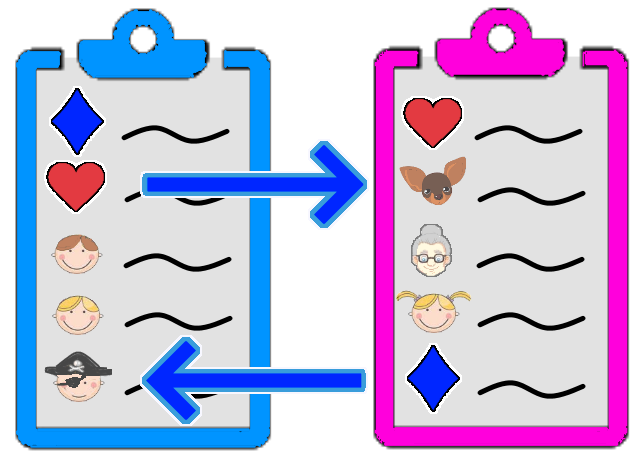
\includegraphics[width=4cm]{Lists.png}}
  \caption{Blue list has a red heart as 2nd. Dog is opposite to it. Pink list has a blue diamond as 5th, same rank as a pirate.}
\end{figure}

Let's see.
\\ I love her the most, then I hang out with my buddy Jake, with my buddy Josh, and I love talking to that homeless beggar every time I go to work.
\\ Wait a minute.
\\ I'm the fourth on the list? Same as the beggar?
\\ I will treat her accordingly!
\scriptsize
* this is not a relationship advice
\normalsize

\subsection{The density: reachability distance}
\epigraph{Zimmel says that freedom is always freedom from something, and, where freedom is not~conceived as the~opposite of restraint, it~is~meaningless. That is so, of course. But~this~slight, elementary truth cannot serve as a~ground for refuting the~thesis, which constitutes one of the~most brilliant discoveries ever made by philosophic thought, that freedom~means~being~conscious~of~necessity.}{G.V.~Plekhanov, On~the~Role of~the~Individual in~History}

Have you ever though about things? What are they made of? What is the density?
\\ Ratio of weight to volume, and that defines the material, right? What if you change the scale, and zoom in. You eventually realize that your object is made of 99\%~"emptiness" and 1\%~molecules.
\\ Your measurement of volume would drastically change, and your density too.
Same material has different densities on different scales.

To overcome this contradiction we will restrict the freedom of choosing the volume. Instead of picking the scale of the volume, we will pick two objects. The shortest distance will produce two points, two radii and two volumes with mass in them. We would be able to tell what volume has more mass, which is denser. Similarly, we use regular density to tell if material will float or drown.
\\ The dialectical distance is our equalizing radius. To get it we need to answer the question: what is the new distance that would have the same amount of mass?

\begin{figure}[H]
  \centering
  \href{\githubPics sun_earth.png}{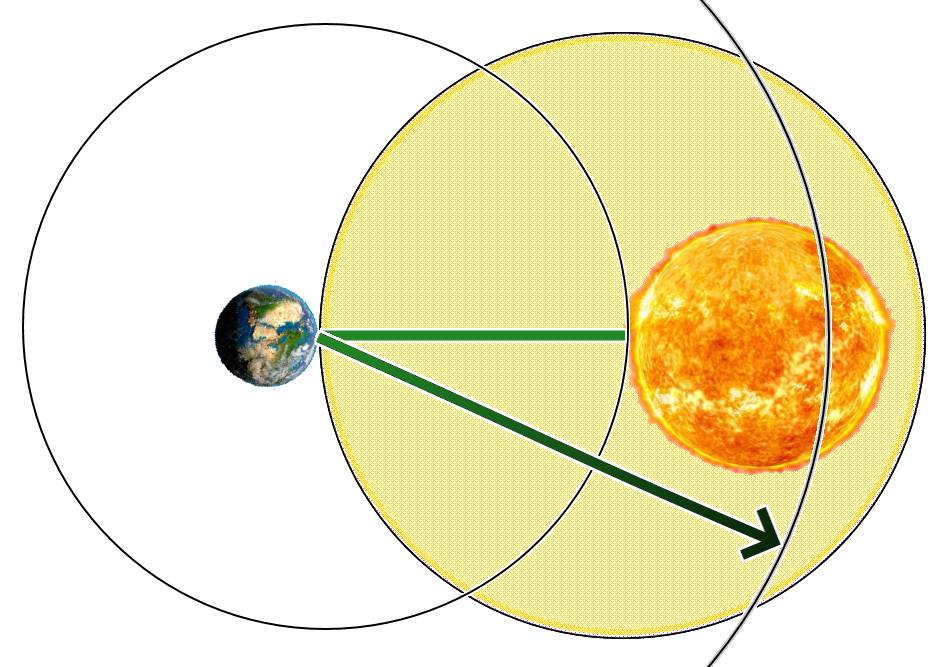
\includegraphics[width=3.5cm]{sun_earth.png}}
  \caption{The shortest distance is the radius for two opposing spheres. Orange sphere has more mass, therefore the other sphere has to be enlarged to devour the same mass. That radius is a dialectical distance.}
\end{figure}

This distance depends on the distance between the points and the difference of the masses. This dependency can be hyperbolized on Sun and photon example (see Figure \ref{fig:photonSun}). Their masses are drastically different and radius extends by about $min(2r, D)$. When photon is far away dialectical distance is a little bit bigger than actual distance. When photon is close to the Sun, the distance will be doubled. The space curves.

% https://tex.stackexchange.com/questions/37581/latex-figures-side-by-side
% http://www.peteryu.ca/tutorials/publishing/latex_captions
\begin{figure}
  \centering
  \begin{minipage}[t]{.45\linewidth}
    \href{\githubPics sun_mid.png}{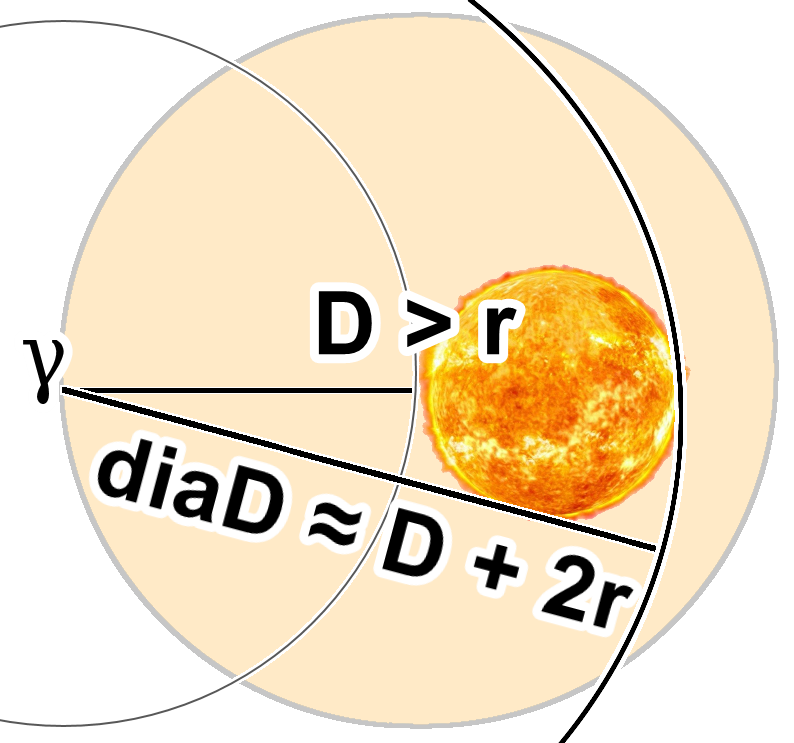
\includegraphics[width=.9\linewidth]{sun_mid.png}}
    \subcaption{Shortest distance is greater than Sun's diameter}
    \label{fig:photonFar}
  \end{minipage}
  \hspace{.02\linewidth}
  \begin{minipage}[t]{.45\linewidth}
    \href{\githubPics sun_close.png}{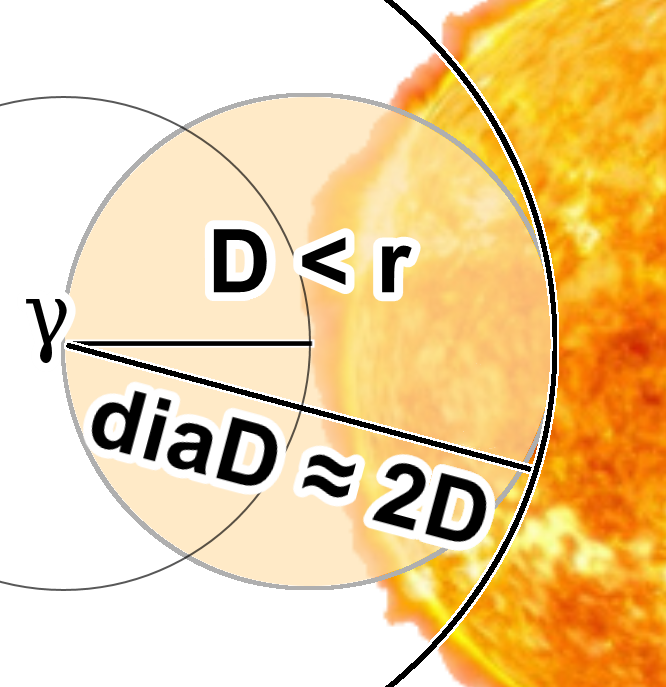
\includegraphics[width=.9\linewidth]{sun_close.png}}
    \subcaption{The object is near the Sun}
    \label{fig:photonClose}
  \end{minipage}
\caption{Evaluation of equalizing radius depending on the position to the Sun}
\label{fig:photonSun}
\end{figure}

In IT we deal with discrete pieces of data. Similarly we could consider drawing radii between points and evaluate how many points are in. The outlier would have only one point, but opposing area many.
This concept is flawedly used in "Local outlier factor"\cite{LocalOutlierFactor} algorithm.
\\ The flaw is in reachability distance that requires parameter $k$ -- it sets the radius to enclose $k$ neighbors. Wrong pick of $k$, leads to bad results. The points themselves produce the $k$, no need to preset it. Without the parameter $k$ reachability distance become the dialectical distance. 

We showed how to strip off a freedoms off ideas to get a better deterministic results.
True determinism necessarily doesn't have any freedoms.
Yet, the freedom of picking the pair of points is still in our way, no worries, it will be taken away later on. There will be no ideas left in our matter.

These examples were the preparation for the opposite direction of development. Instead of stripping we would have philosophical growing from the bottom to the top. Ascension of abstract beings through their relationships to the definite entities.

\subsection{The subject: contradictions}
\epigraph{There is only one subject, the~world~as~a~whole}{Basis of dialectical materialism}

The subjects exist. They are independent in their subjectiveness. Every subject independently examines its' relations to other subjects. For convenience consider the example below.

\begin{figure}[H]
  \centering
  \href{\githubPics Closest.png}{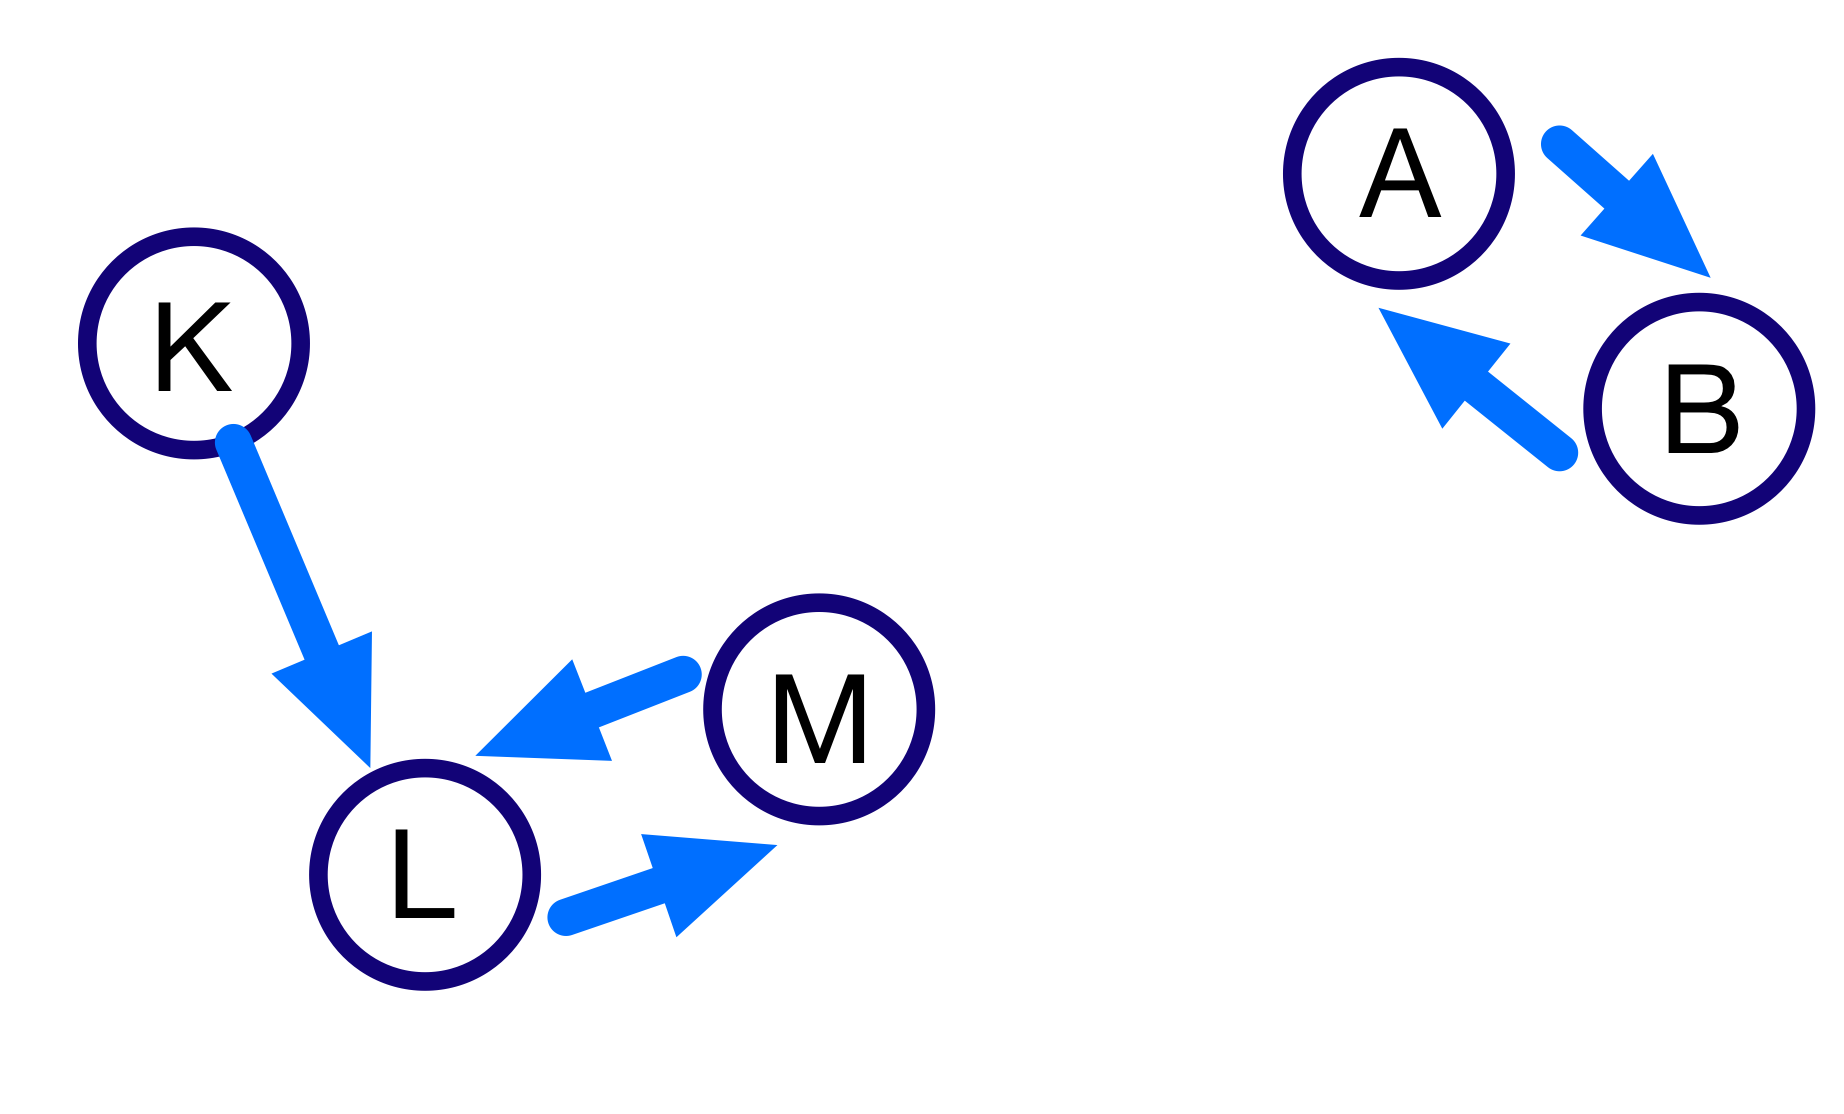
\includegraphics[width=3.5cm]{Closest.png}}
  \centering
  \caption{Marked subjects where arrows denoting the closest neighbors for the subject.}\label{fig:Closest}
\end{figure}

Each subject has many relations but one of them is particular -- a closest one.
\\ Mutuality of closeness is not guaranteed as it is shown in example with subjects K and L.

\begin{table}[H]
\caption{What is happening between K and L?}
\begin{tabular}{ p{3.8cm} | p{3.8cm} }
  \hline
  If K would rank it's closest relations: & If L would count from itself: \\ 
  \hline
  1. K is first & 1. L is first \\
  2. \textbf{L is second} & 2. M is second \\
  3. M is third & 3. \textbf{K is third} \\
  ... & ... \\
  \hline
  \href{\githubPics Count.png}{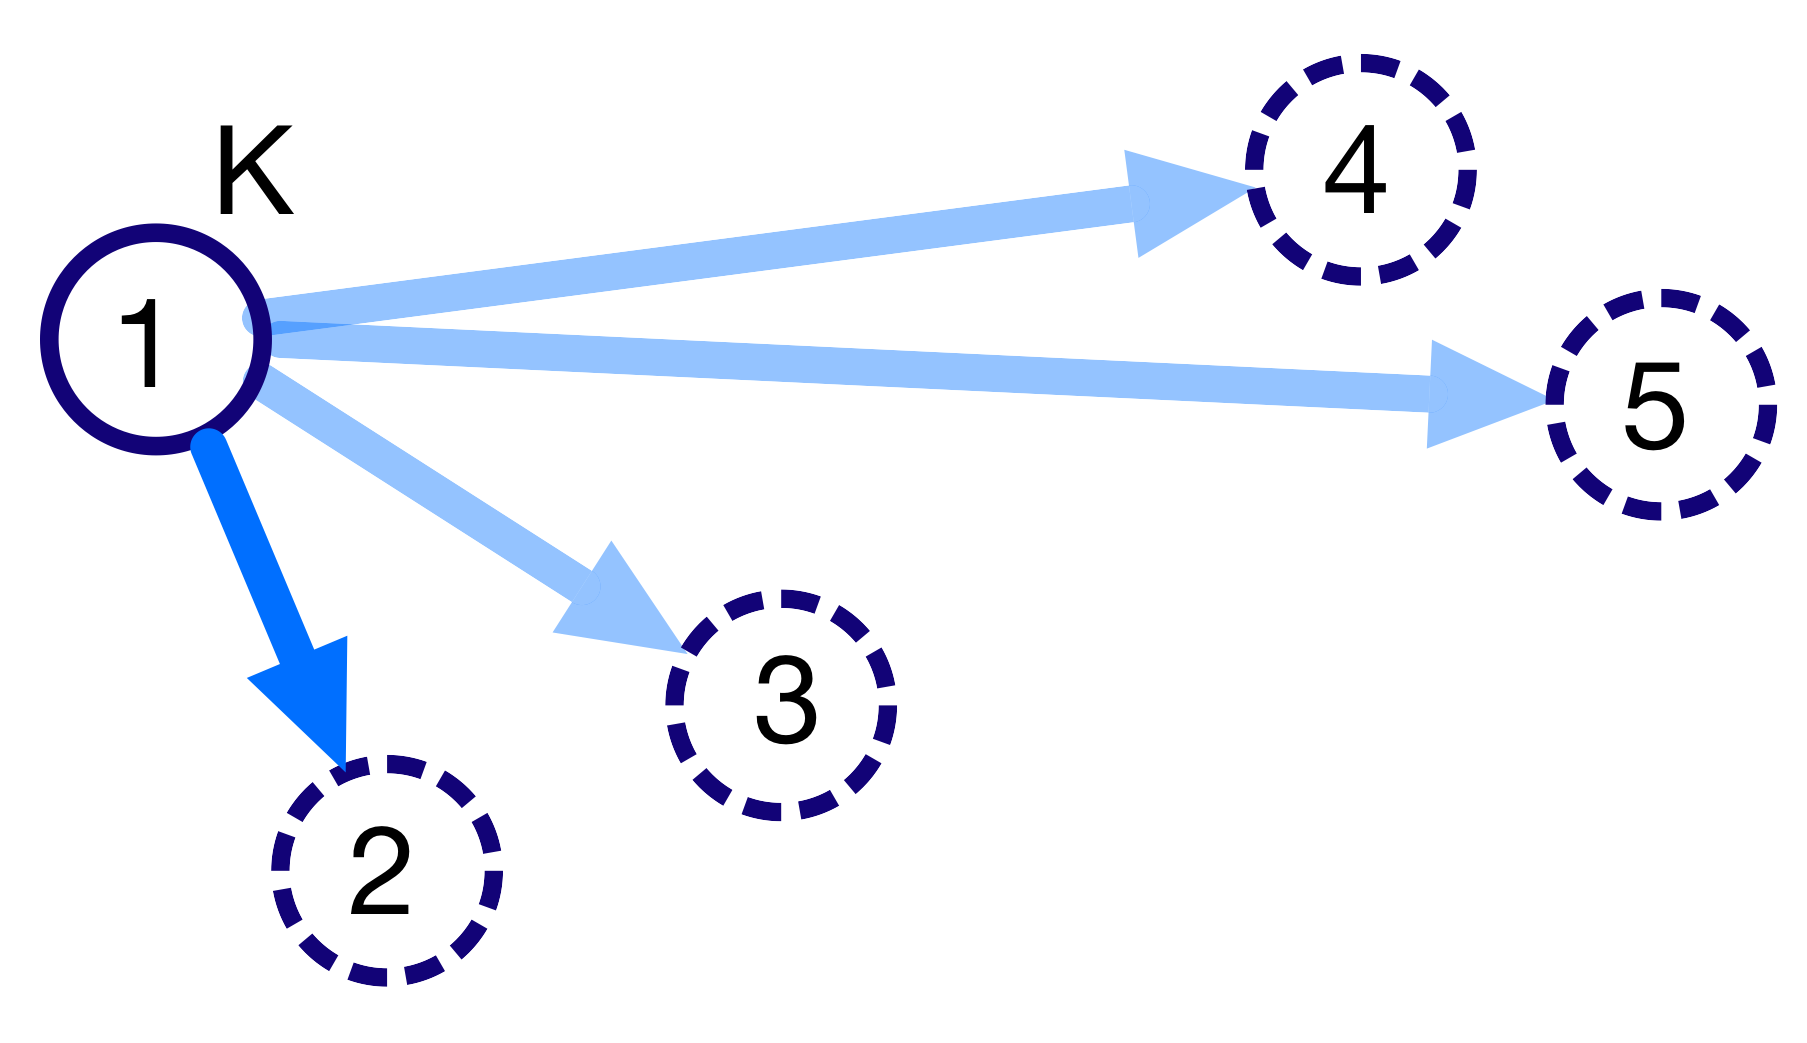
\includegraphics[width=3.5cm]{Count.png}}
  $Rank_{KL}$ = 2 
  & 
  \href{\githubPics Count_2.png}{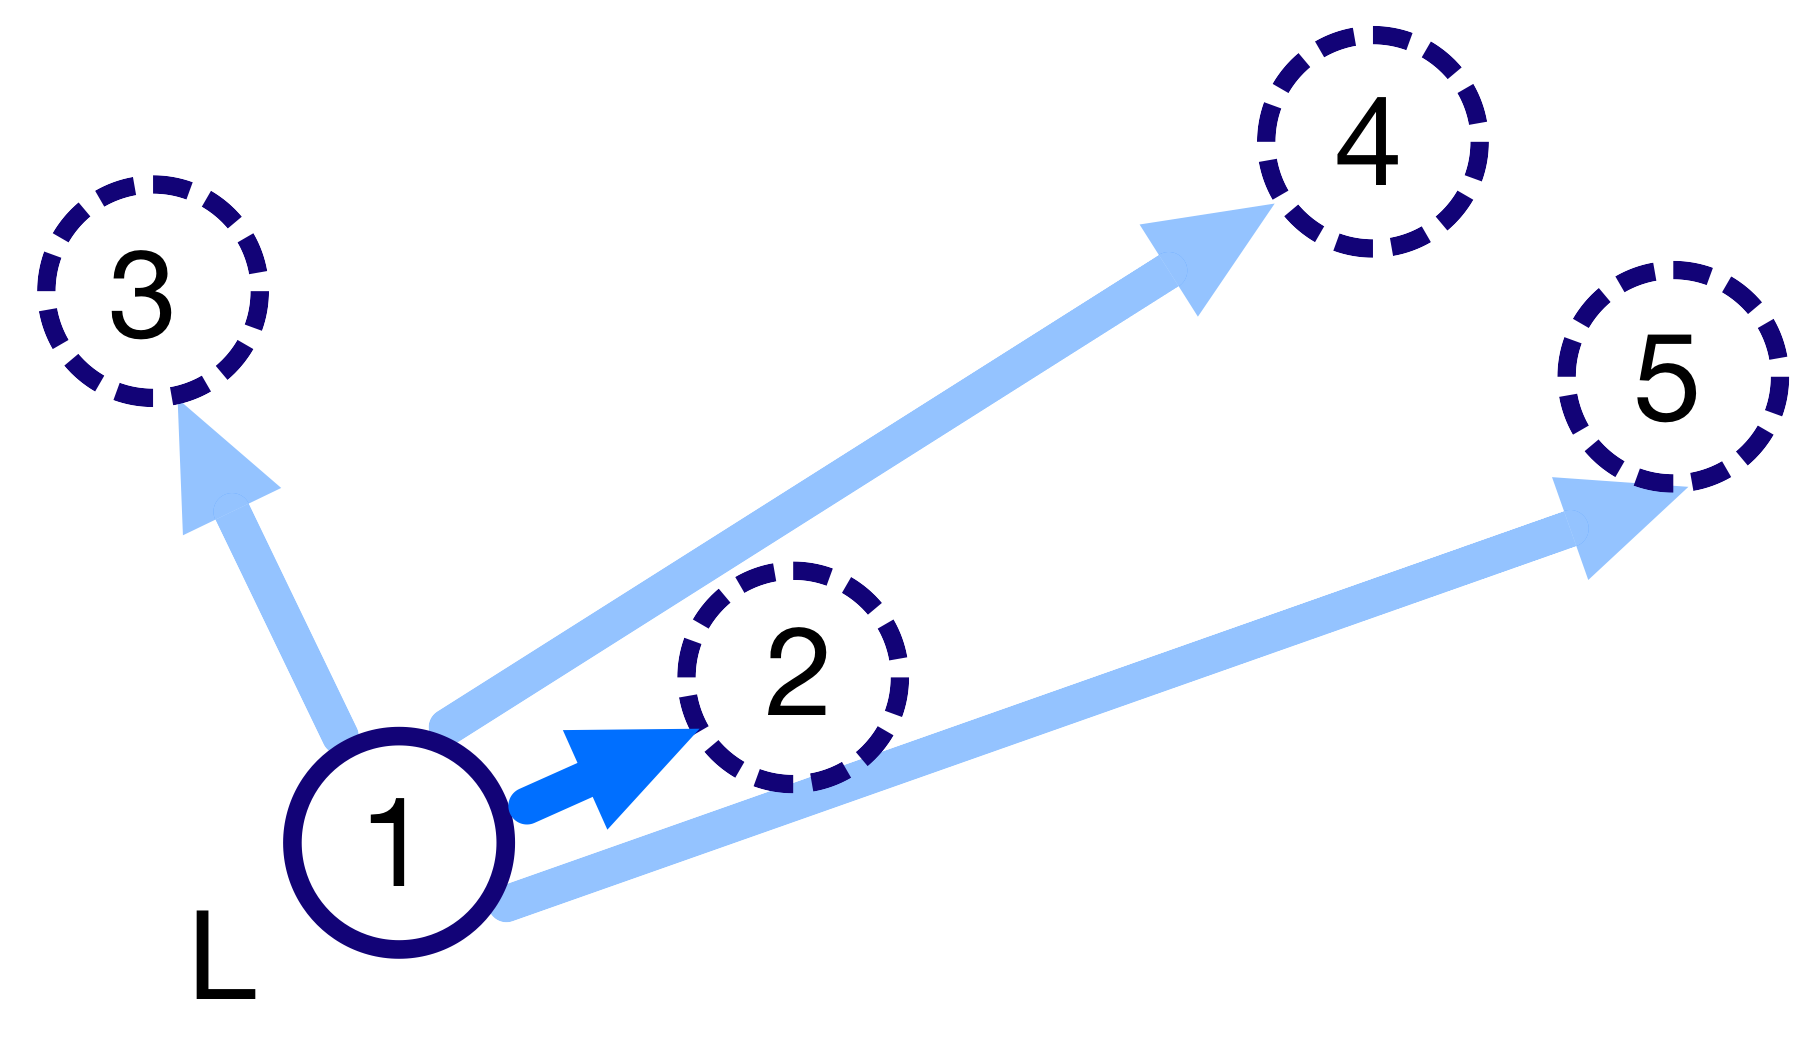
\includegraphics[width=3.5cm]{Count_2.png}}
  $Rank_{LK}$ = 3 \\
  \hline
\end{tabular}
\end{table}

\begin{figure}[H]
  \centering
  \href{\githubPics Count_3.png}{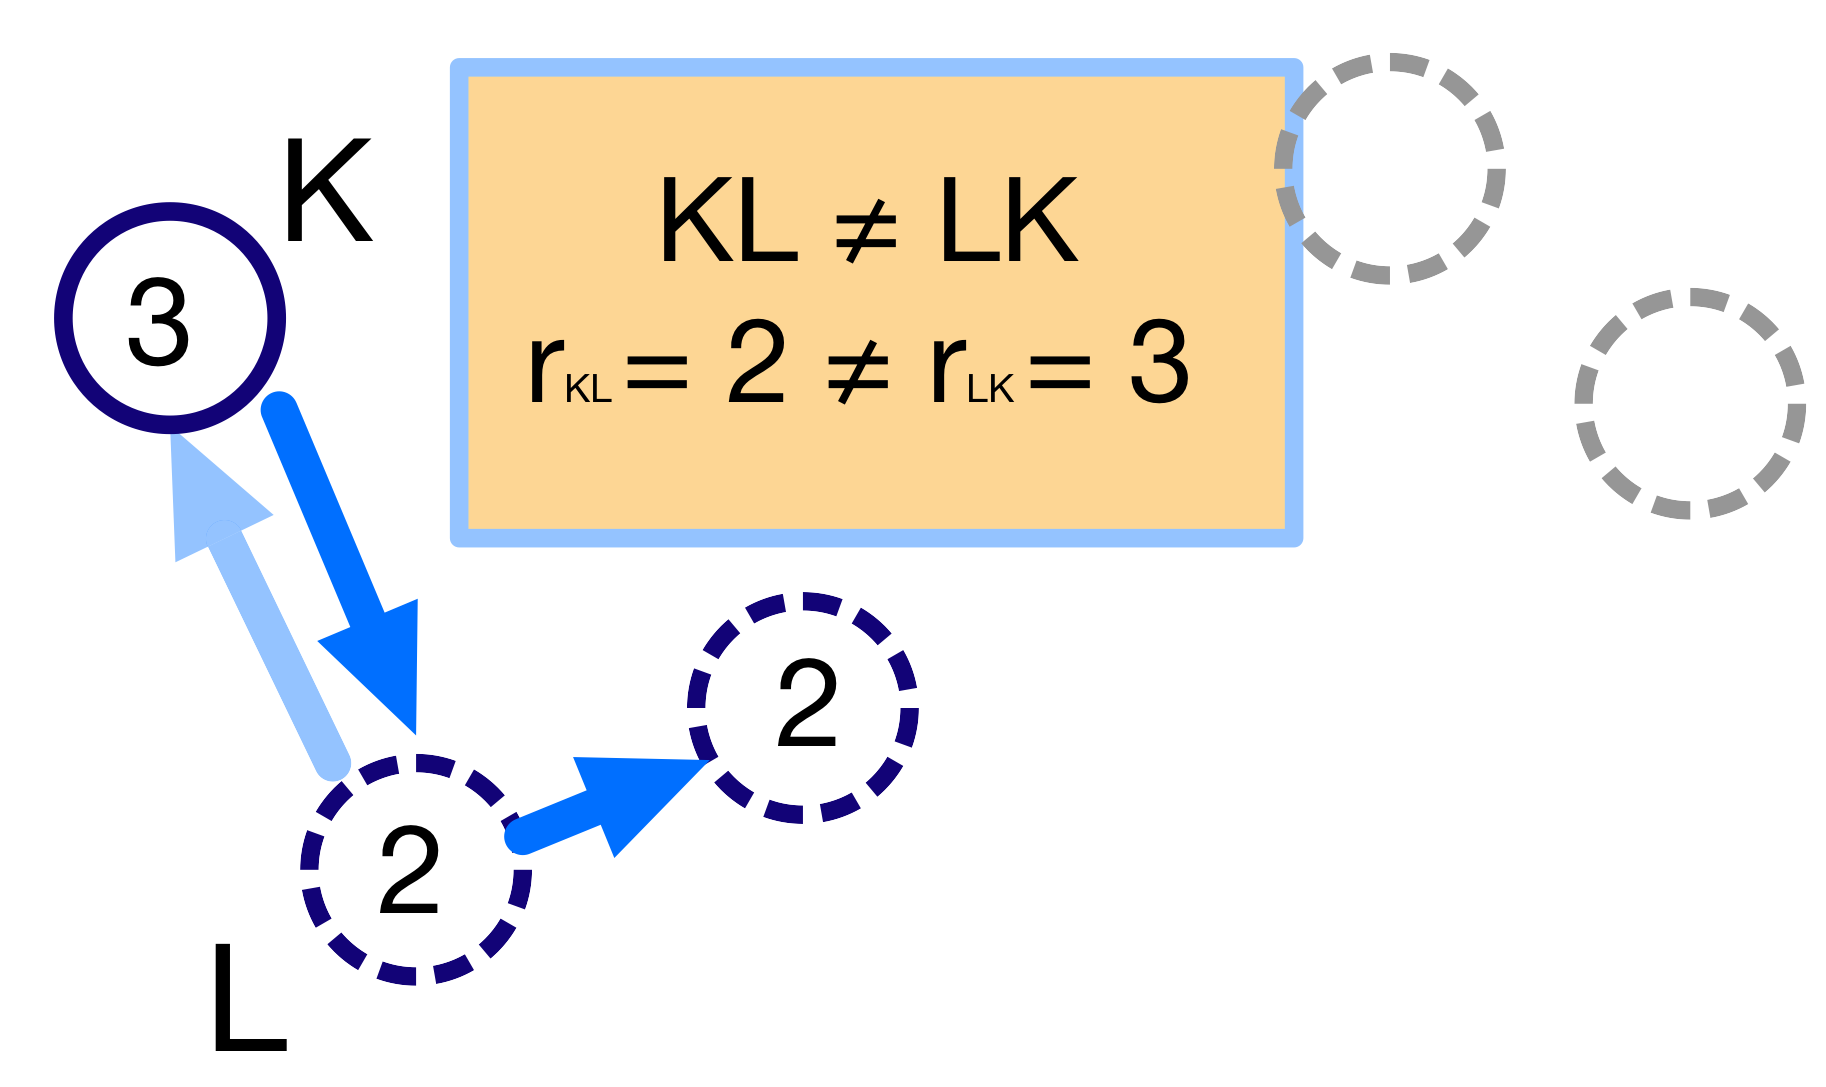
\includegraphics[width=4cm]{Count_3.png}}
  \centering
  \caption{For the relationship KL the distance is the same but closest and ranks are different}
\end{figure}

Closest relations can be mutual (like LM, AB), then ranks and distances would not cause the contradictions.
\\ Contradiction appears in relations that closest/particular in one direction and not particular, not closest, but indifferent in the other direction(like LK).
\\ \textbf{Same relationship is particular/closest and not at the same time.} That is a contradiction that has to be negated(positively resolved).

Let's examine this relationship from two opposite sides quantitative and qualitative: \\Quantities-ranks do not match 
\vspace{\myvspace}

\centerline{$Rank_{KL}~\neq~Rank_{LK}$}
Qualities-distances do match at the first glance. Only at the first glance. Category \textit{quality} means internal properties, they are not accessible to external observer. Qualities cannot be transferred!
\\ Subject K doesn't know how he is perceived by L. He can reconstruct it by counting his rank in L's numeration and he can see that it doesn't match his enumeration. He could fix that: \ul{To get other's quality you need to get your quality of other's quantity.}
\\ Then the qualities of both parties would be equalized from their point of view and the contradiction will be resolved.

\begin{figure}[H]
  \centering
  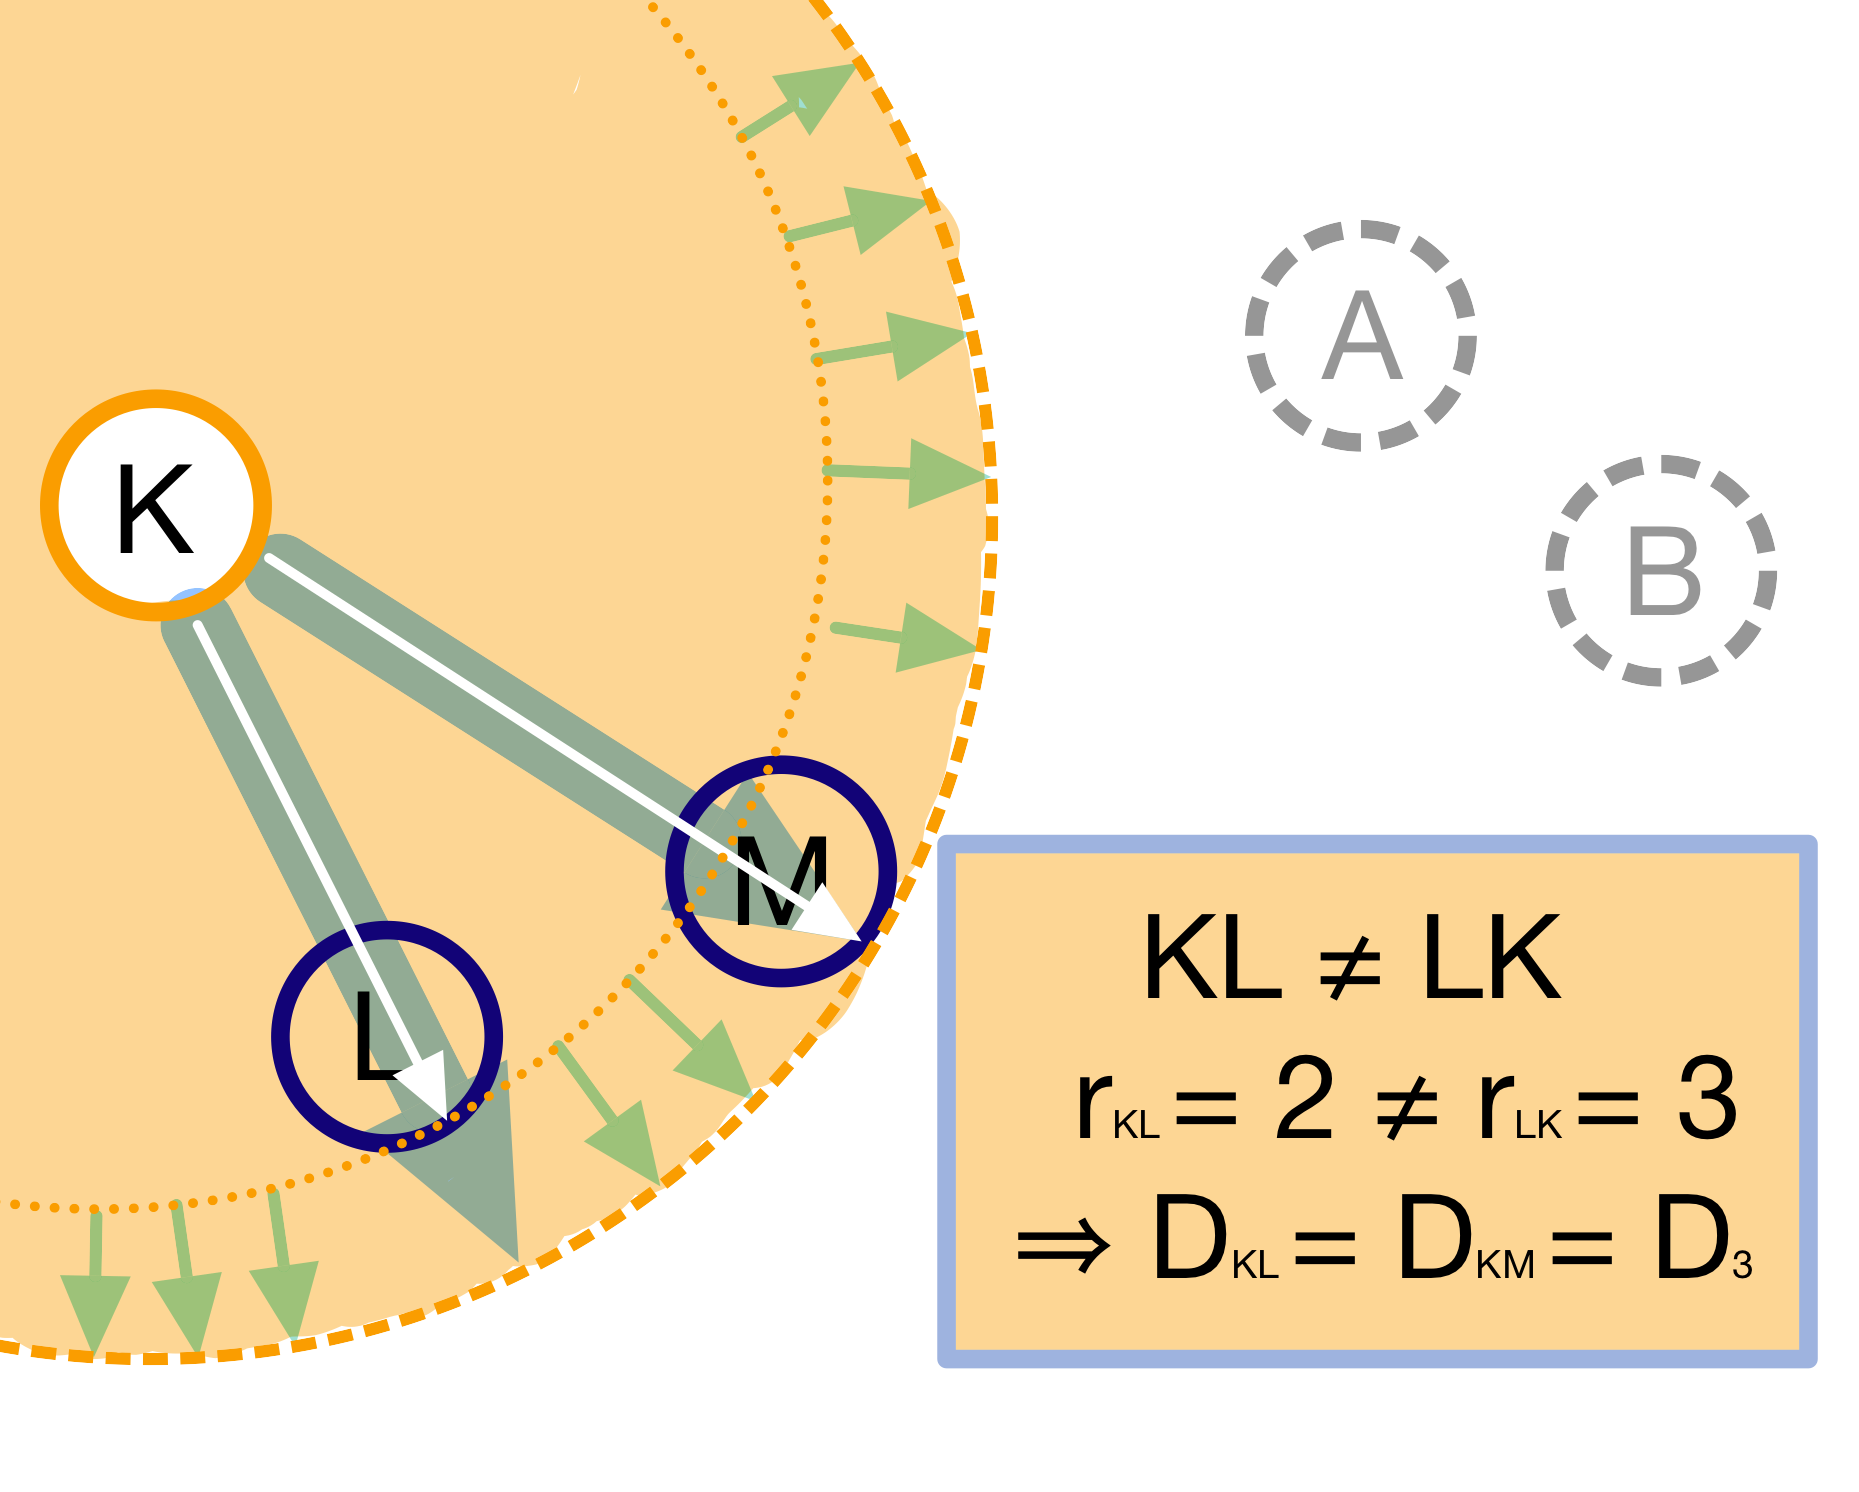
\includegraphics[width=3.5cm]{Increased.png}  
  \\ $ D_{KL} = d_{KM} = d_{3} \neq d_{KL} $
  \caption{The distance from K to L would extend to the third rank. Instead of white thin line it pierces through as thick bold.
  \\ Colored area has equal indifference.}
\end{figure}

The subject K relate to L same as to M. In it's opinion L treats him that! 
\\ And now, for K distance to L and M is of the same particularity, relation to a subject dissolved and gave birth to the relation to something else.

\section{Bridging the Amalgamation}
\epigraph{Struggle and unity of opposites}{Law of dialectics}
% \section{Ordered emergence}

Usually it would be an end of it. Having dia-distance, we could build a graph out of it. Find shortest paths and gradually connect nodes into bigger and bigger subgraph until we achieve a graph-tree. That would be wrong! We can't operate amalgamated subgraphs, which we didn't define, that's an extra information to avoid.

Direct defining is a new info. Instead, new entity should be developed from the Subject and it's relations. To prevent contamination by external \textit{ideas} we need to use dialectics\footnote{More on dialectics read in appendix\ref{On dialectics}}. We are going to analyze quality and quantity and then embrace them and ascend to the next order of entities. We will show how graphs came to be.

Dia-distance of the relation is it's qualitative part. It's inner part. What would be it's counterpart?
\\ It's outer part? Amount of Subjects, it's rank, it's quantitative part. What would be it's counterpart?
\\ It's inner part -- dia-distance. We found two contradictions that are made by negating each other.
\\ Repeating the negation goes to the bad infinity.

The radical change of the view gives a different result of the same object. The negation provides that view for the complete coverage of the object. Two Qs are as different as possible, and at the same time are making the whole, that is confirmed by bad infinity. We want even more radical change the change in entity.

To break away from the bad infinity we have to negate the unity of Qs. That unity should be denoted as the context, that whole. And at the same time, the context should lead to the next level whole -- Amalgamation.
\\ The bridge between Subject's relation and Amalgamation is a Measure(of membership), the Subject would try itself as a part of the party. On one bank of the relation it's members M and on the other 1 member. The membership is a subjective and like a quality cannot be perceived by outsiders, therefore other membership is always look like a loner 1(no extra ideas about the size of the opposite group).
\\ The measurement is almost a new entity. Subject already feels as an Amalgamation. Acts instead of it and for it. % Действует за неё и для неё.

\begin{figure}[H]
  \centering
  \href{\githubPics Triada.png}{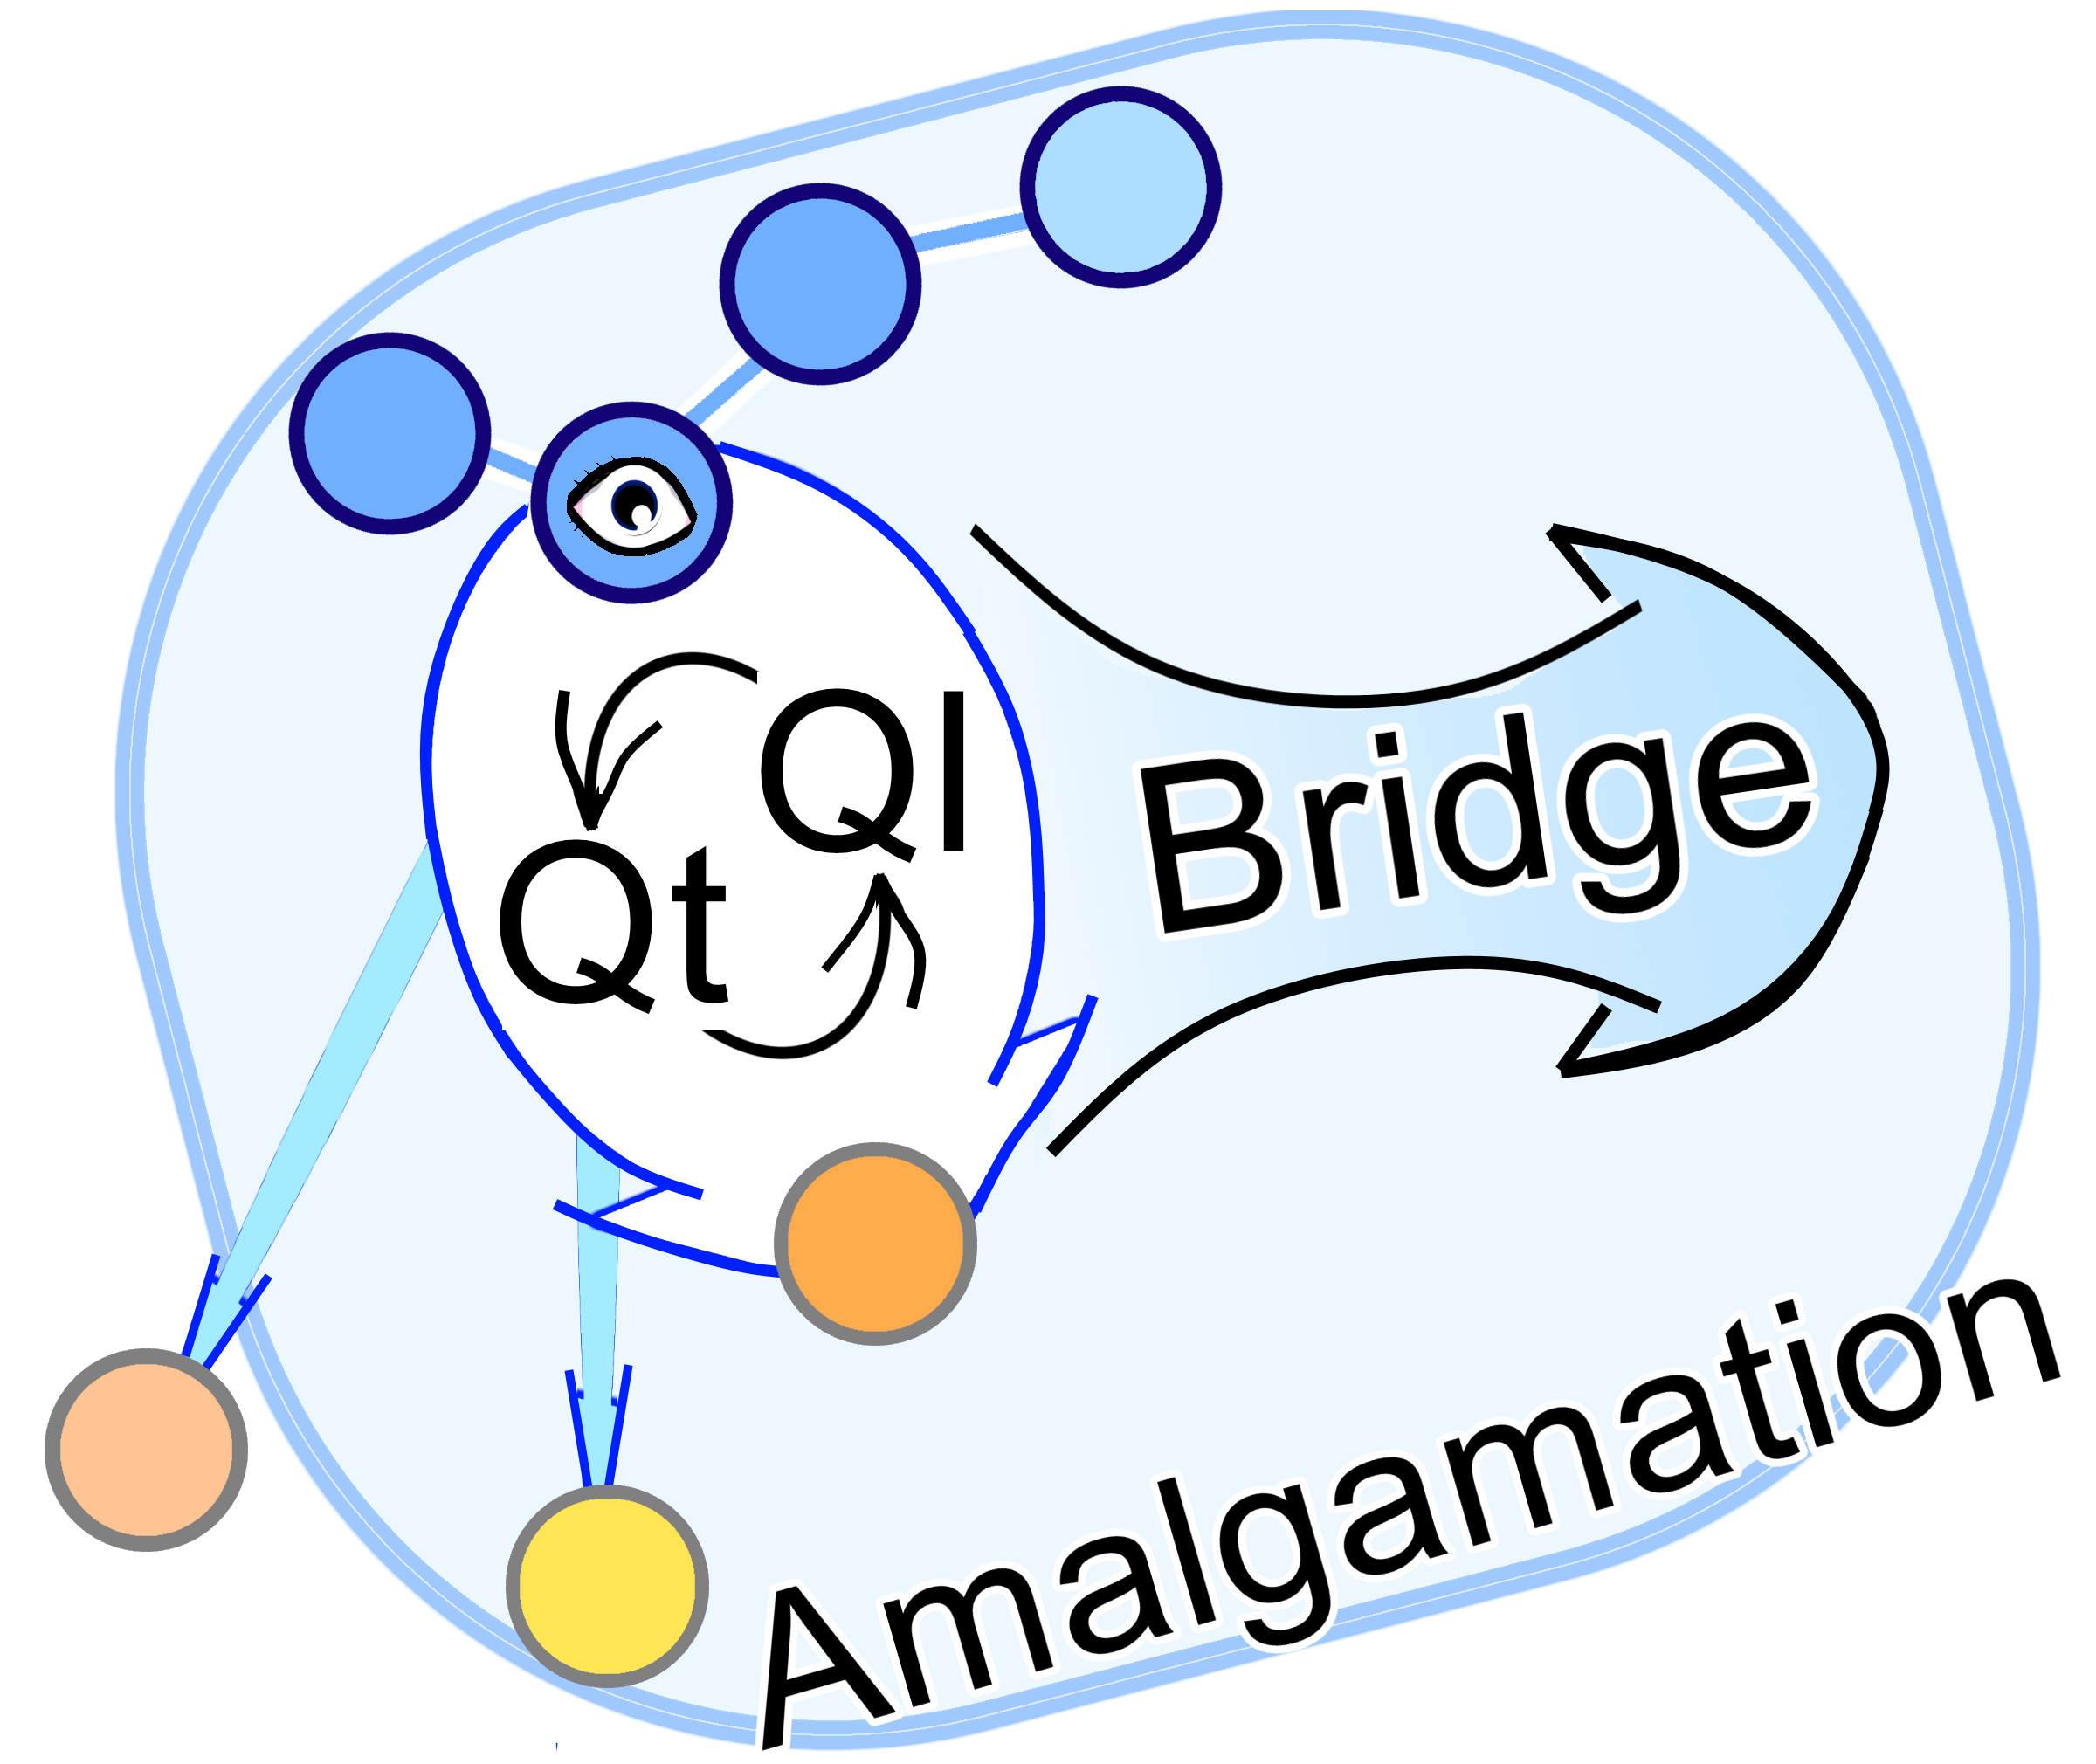
\includegraphics[width=3.5cm]{Triada.png}}
  \centering
  \caption{The Subject(eye) perceive the surrounding. It relates to Others. The relationship has contradictory inner and outer components. The Bridge helps to negate it to the level of Amalgamation.}
  \label{fig:Triad}
\end{figure}

On Figure \ref{fig:Triad}, the bad infinity of Qs and Bridge that overflows to the Amalgamation. The solidified relation is an edge that builds the graph. Mathematically speaking, terms Ql-Qt+Bridge become the expression\footnote{Technically speaking, the degrees help with tiebreaks(more info in examples\ref{Examples})}:
\vspace{\myvspace}

\centerline{$r \cdot D^2_r \cdot \sqrt{\frac{M+1}{M \cdot 1}} \rightarrow min$}
\begin{itemize}
\item $r$ -- rank (quantity)
   \\ $r \geq R$ (R is my counting to other)
   \\ \textit{least rank, comes first}

\item $D_r$ -- dia-distance (quality) 
   \\ my distance of other rank $D_r \geq D_R = d_r$ (original dis)
   \\ \textit{closest, comes first}

\item $\frac{M+1}{M \cdot 1}$ -- membership (bridge)
   \\ M is my members in my R-vicinity
   $1 < \frac{M+1}{M \cdot 1} \leq 2$ (it can be ignored with big M's)
   \\ \textit{higher membership, comes first}
\end{itemize}
Solving the optimization problem for all edges produces Minimum Spanning Tree(MST) (Fig. \ref{fig:Ordered}). Similar environments("densities") connect first and the outliers at the end. Mathematical part of first phase has ended.

\begin{figure}[H]
  \begin{minipage}[c]{0.40\linewidth}
    \href{\githubPics Ordered.png}{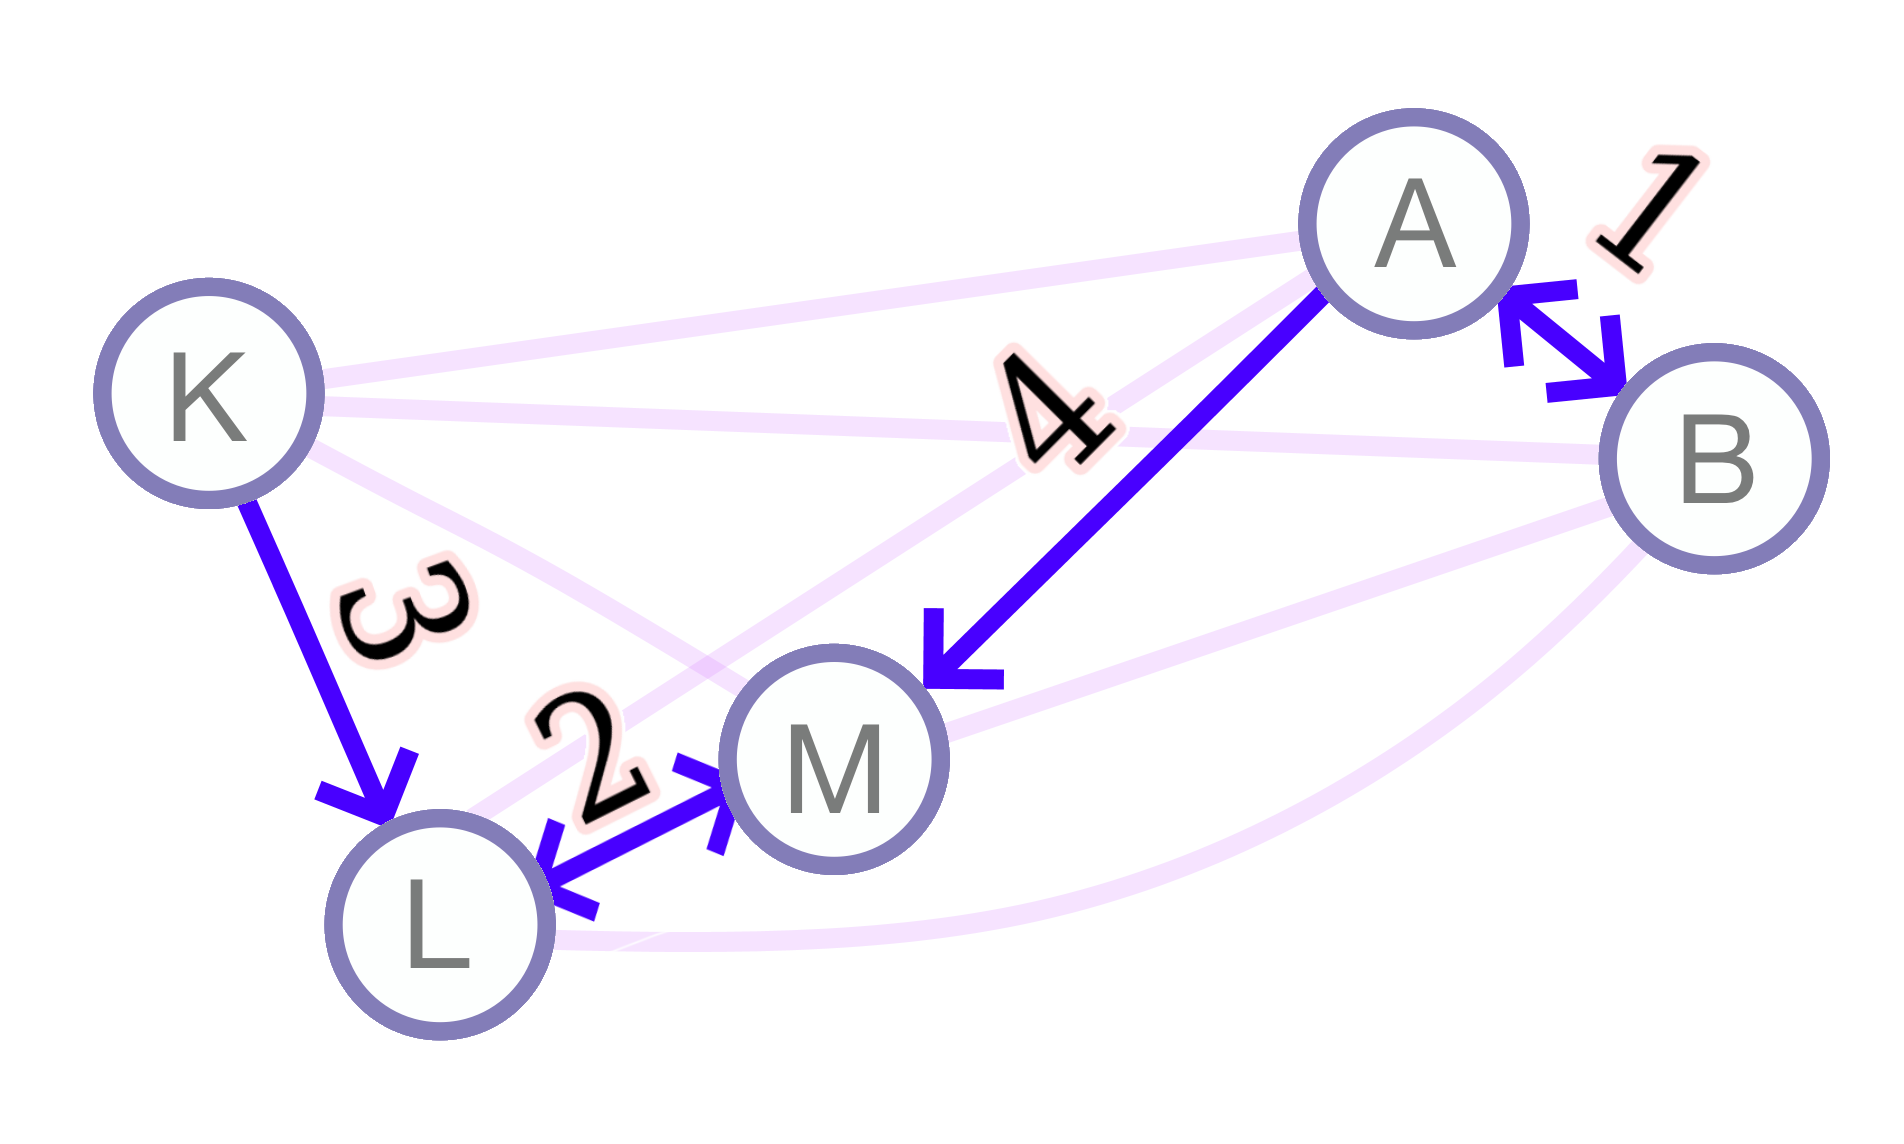
\includegraphics[width=\linewidth]{Ordered.png}}
  \end{minipage}\hfill
  \begin{minipage}[c]{0.60\linewidth}
    \caption{The ordered directed connections form MST. Lighter edges lost the struggle of the opposites signaling the end of first phase.} \label{fig:Ordered}
  \end{minipage}
\end{figure}

The philosophical part echoes. The opposites that struggles is the relationships of one Subject, and not the contradictions of relation. The struggle overflows to all Subjects. On one hand, Subject doesn't care about other side's connections and amalgamations, on the other hand, he senses the inequality through dia-distance and have to "wait" for closer connections. After the merge the other side connections revealed to him, meaning they existed prior the merge. The local relations are clearly independent, like 1 and 2 relations on Fig. {fig:Ordered} their global order can be exchanged without an effect. On the contrary, the highest connection 4 cannot change it's order, it has to be the last. Like that subjectives of singular becomes the objective universal. 

The one by one reveal of particular relationship of all singulars sticks into the single universal.

\section{Cluster -- the particular Amalgamation}\label{sec:Cluster}
\epigraph{Transition of quantitative changes into~qualitative~changes}{Law of dialectics}

The outcome of a previous phase, was the subjective relationships solidifying into Amalgamations. Formed Amalgamations were uniting and like a rolling snowball growing into one huge Amalgamation. The Subjects were seeking the Universal. 
\ul{Uniting to become a part and not a whole?} This contradiction between singular and universal is transcended by particular. In other words, Amalgamation can become it's own whole -- the cluster. Once a cluster -- harder it takes to change it.

\begin{figure}[H]
  \centering
  \href{\githubPics Cluster.png}{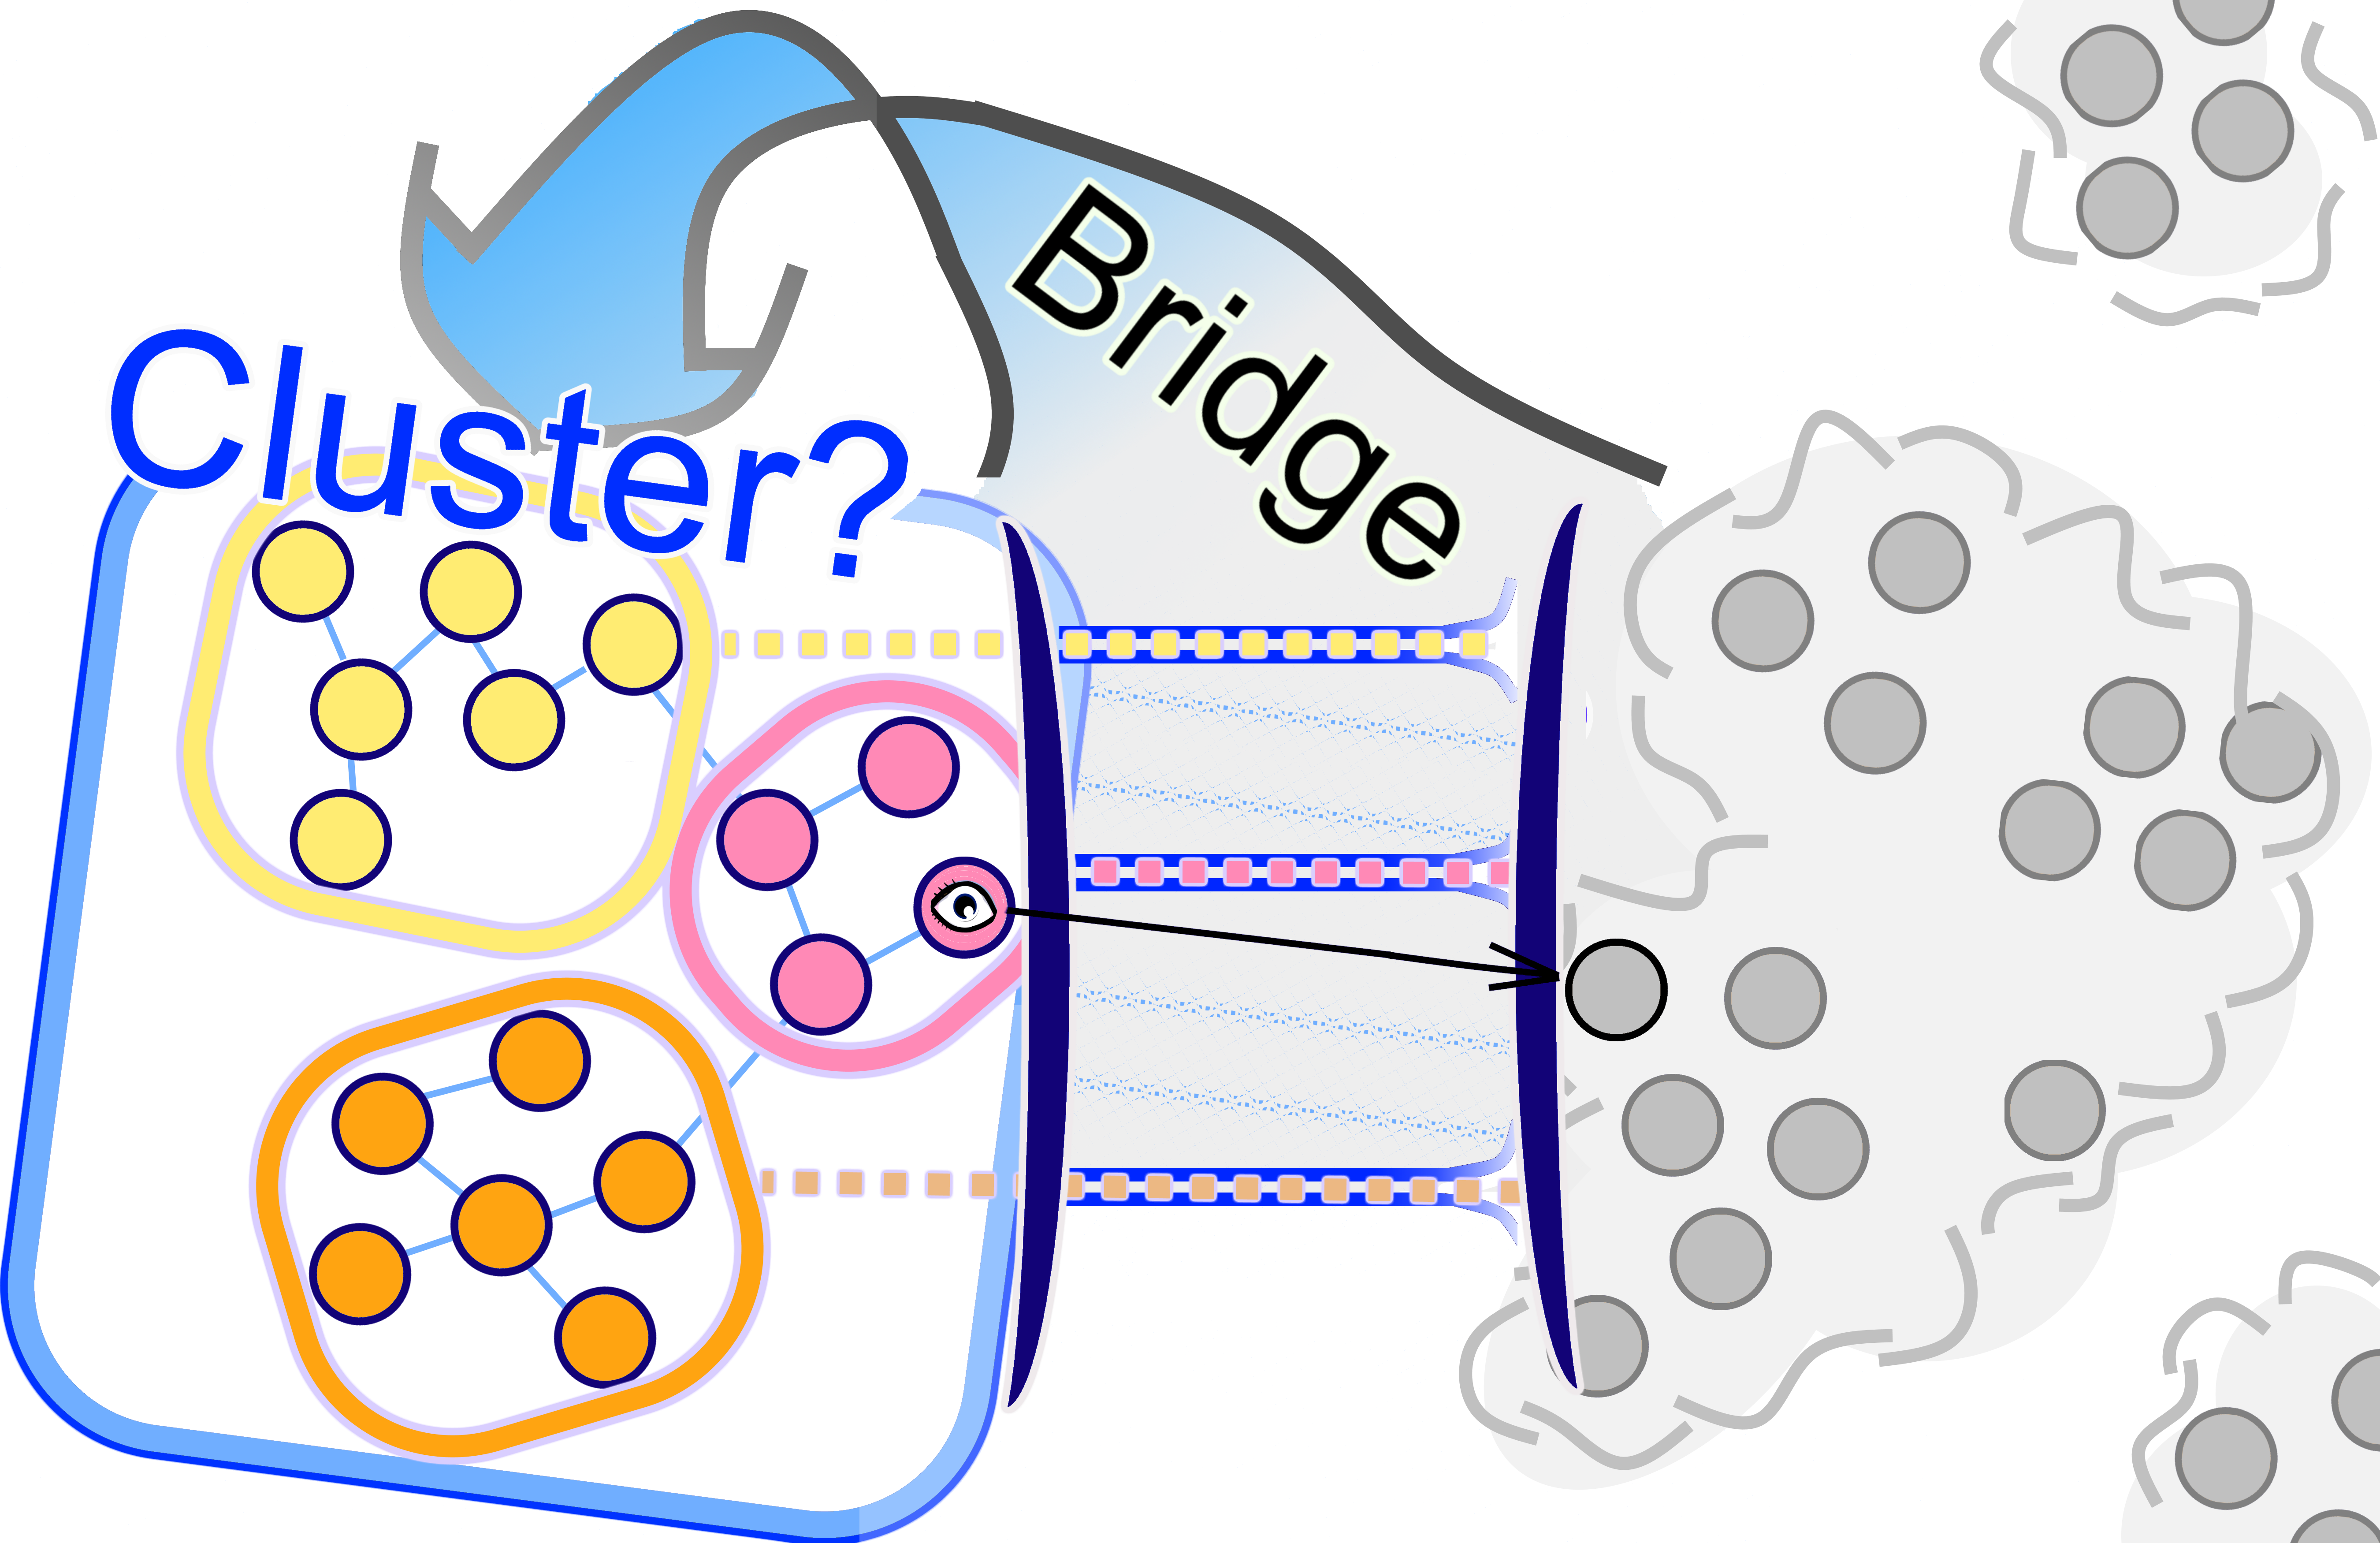
\includegraphics[width=3.5cm]{Cluster.png}}
  \centering
  \caption{Amalgamation of colored clusters is halted by Border. Border's area(dia-distance times clusters' streams) can wrap a new Cluster. The Bridge helps with sides' count.}
  \label{fig:Cluster}
\end{figure}

The \textit{border}(Fig. \ref{fig:Cluster}) connects and divides Amalgamations(subgraphs). It is in and out of Amalgamation, it stops the advance of unification. The internals face external limit, if it's significant enough then Amalgamation was/become a Cluster.
\\ Can we(the Clusters) overcome it and unite? The Border relation:
\vspace{\myvspace}

\centerline{$K \cdot D^2 \cdot \sqrt{\frac{N \cdot n}{N + n}}$ } % желательно поместить это на одну страницу с подобной формулой.
\begin{itemize}
  \item $K$ —- my clusters (quantity)
    \\ can't "perceive" other side's clusters
    \\ \textit{more clusters, more a mix looks as One}
  \item $D$ -- dia-distance (quality)
    \\ the Border is "perceived" by Subject
    \\ \textit{more standing out, more distinct it looks}
  \item $\frac{N \cdot n}{N + n}$ -- gain (bridge)
    \\ acts as continuous $min(N, n)$
    \\ It's the growth of the Whole. It bridges Amalgamation(and it's parts) level to the level of Universal/Whole. For Amalgamations merge is a unity, for the Whole it is an addition of a smaller.
    \\ \textit{outliers won't matter}
\end{itemize}

The new Cluster will emerge after the overcoming of internal limits, if
\vspace{\myvspace}
\centerline{$\sum_K N_{i} \cdot D^2_{i} \leq K \cdot D^2 \cdot \sqrt{\frac{N \cdot n}{N + n}}$,}
then all internal differences erase and identity flushes for each Subject. Externals replace internals and each Subject's new limit is $D^2$ and Cluster's limit is $N \cdot D^2$.

The Clusters reflect to themselves of the border and gain another identity. The self-reflection grants them capacities of a border's limit. The capacity represented by Subject's view by the dia-distance.
\\ This complete replacement of the previous limit in practice solves the problem of spurious outlier's contribution. In a regular density algo, even one super-dense relationship (a density $1/dis$ can be infinite) could drag entire cluster's attributes down. To fight that, algos introduce smoothness parameters that complicate cluster extraction. The DRUHG avoids extra \textit{ideas} all along.

\begin{figure}[H]
  \centering
  \href{\githubPics Nested.png}{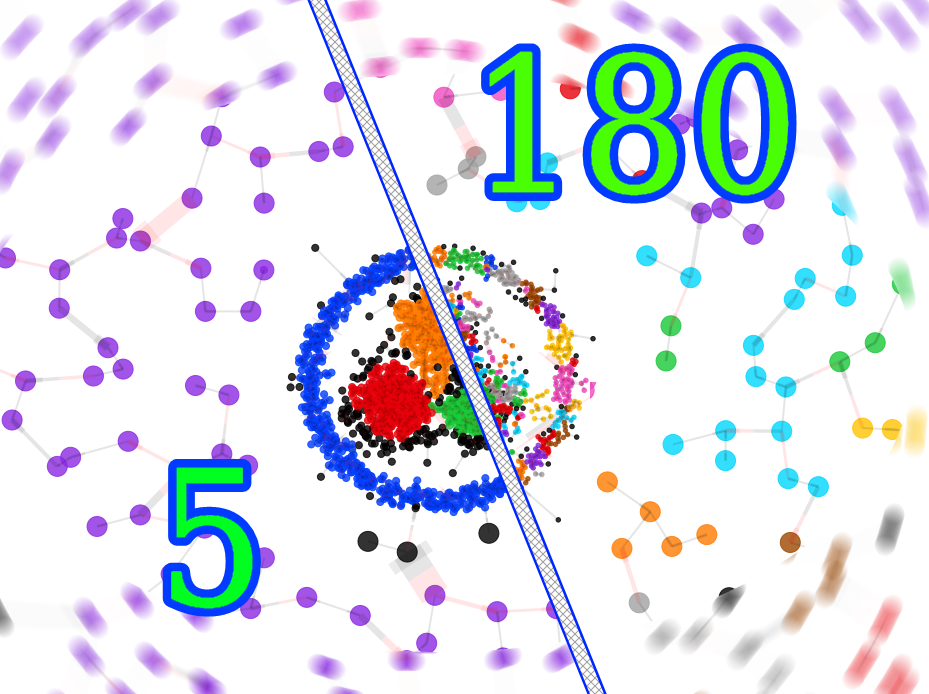
\includegraphics[width=3.5cm]{Nested.png}}
  \centering
  \caption{Autopsy on the different scales. Left side has 5 clusters. Right side dissects clusters and surface the internal clusters.}
  \label{fig:Nested}
\end{figure}

The datapoints start with zero limits. The Border leads them to the clusters. The clusters negated by bigger borders into bigger clusters. Until the last link connects them to One Universal Amalgamation but never in one cluster. The clustering is complete, you as an observer can access it's nested structure (Fig. \ref{Nested}).

\section{Two phases comparison}
\epigraph{The chief forms of beauty are order~and~symmetry~and~definitenesss, which~mathematical~sciences demonstrate~in~a~special~degree.}{Aristotle}

Let's compare both phases and highlight some interesting facts. 

The formulas' components Ql-Qt-Br are stunning with the symmetricity. \centerline{$r \cdot D^2_r \cdot \sqrt{\frac{M+1}{M \cdot 1}}$ vs $K \cdot D^2 \cdot \sqrt{\frac{N \cdot n}{N + n}}$} The qualities are the same, they are sensed through the same Subject. The difference comes from the order of the entity phase operates with. Quantities of fellow Subjects vs of fellow Clusters. Naive bridging by limiting Amalgamation members with rank-sphere vs limiting Universal with a current connection.

First phase operates with one directional logic of a seeking Subjects. The counter-subject does not seek anything. At the end of the phase, unified Universal emerges, that do "see" the both sides of the merge. So the second phase is symmetrical and the formula is applied twice. The actors are clusters instead of the Subject.

The formulas are independent of a constant factor, e.x. multiplication by $2\pi$ would not change anything.

The figure \ref{fig:Triad} shows bad infinity of Q-contradictions and the other Fig. \ref{fig:Cluster} shows area as the product. Actually, both phases have all of it.

\section{Experiments}\label{Examples}
\textbf{Data Sets.} We report the performance on toy sklearn datasets, Chameleon dataset, synthetic geometric datasets. We used Euclidean distance on all of them.
\textbf{Algorithm.} The code is publicly available and can be run in couple lines of code. Pseudocode and optimization tricks are discussed in appendix\ref{Pseudocode}. The tests run on python version \textit{druhg 1.2.1}.

We will be going through different examples, keep in mind that DRUHG does not require parameters. Other algorithms do. To be fair, we do use parameters for performance boost, that's the k-neighbors limiting the "view" of each subject/datapoint.

\begin{figure}[H]
  \centering
  \href{\githubPics example_chameleon.png}{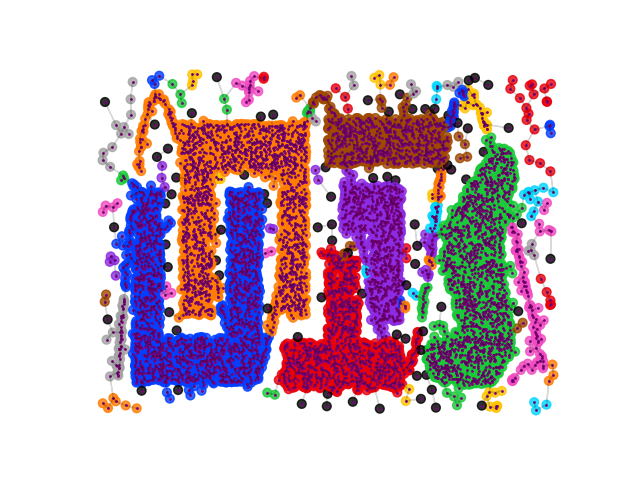
\includegraphics[width=7cm]{example_chameleon.png}}
  \caption{Chameleon dataset.}
\end{figure}
DRUHG could do what DBSCAN can not -- catch clusters with different densities. It did it in one run -- it takes HDBSCAN 5+ runs.  

\begin{figure}[H]
  \centering
  \href{\githubPics example_comparison.png}{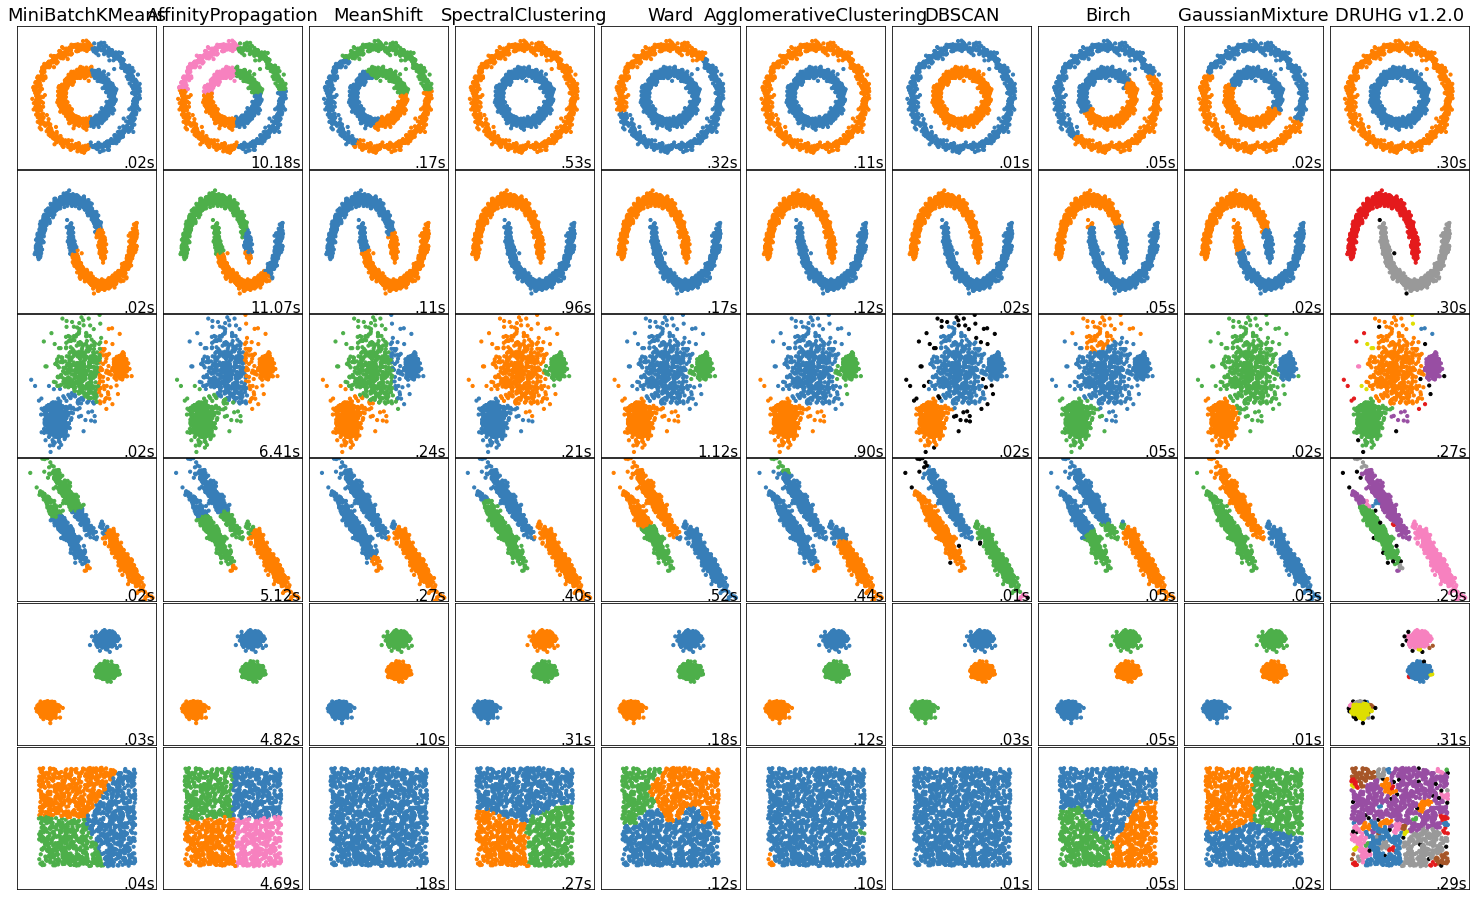
\includegraphics[width=7cm]{example_comparison.png}}
  \caption{Toy sklearn datasets comparison. Last column is DRUHG.}
\end{figure}
The results speak for themselves. Some special things to notice. DRUHG managed to catch individual outliers and small clusters. (Bottom right) It could not catch "cluster-dataset" -- it is not possible to define Being without Other.

\begin{figure}[H]
  \centering
  \href{\githubPics example_diffNNs.png}{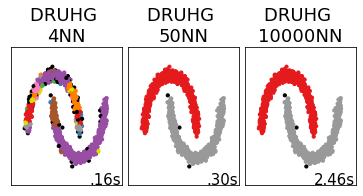
\includegraphics[width=7cm]{example_diffNNs.png}}
  \caption{Performance vs precision. Low near neighbors count (4NN) is not enough for moons confronting each other to form clusters.}
\end{figure}
You can improve performance by decreasing the amount of near neighbors to look at. By increasing the parameter you will increase time and the result will not change at all after a reaching of a certain spot.

\begin{figure}[H]
  \begin{minipage}[c]{0.20\linewidth}
    \href{\githubPics example_line.png}{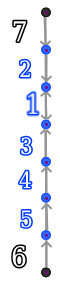
\includegraphics[width=0.4\linewidth]{example_line.png}}
  \end{minipage}\hfill
  \begin{minipage}[c]{0.40\linewidth}
    \href{\githubPics example_square.png}{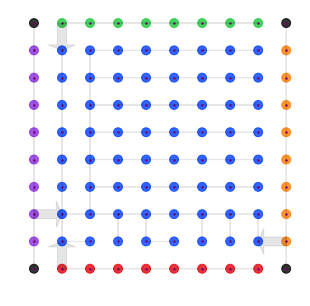
\includegraphics[width=\linewidth]{example_square.png}}
  \end{minipage}\hfill
  \begin{minipage}[c]{0.40\linewidth}
    \href{\githubPics example_cube.png}{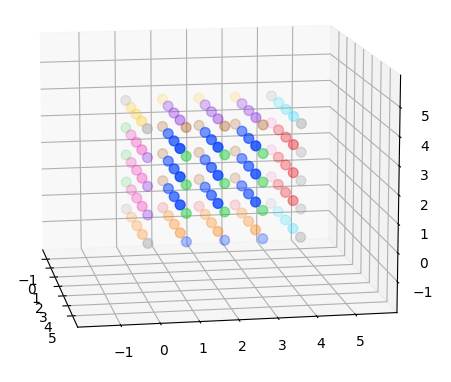
\includegraphics[width=\linewidth]{example_cube.png}}
  \end{minipage}
  \caption{Line, square, cube made of equidistant grid points. Numbers depict the order of connection.}
\end{figure}
DRUHG defined vertexes, edges, faces, like human does. Line starts from any of the body links, everything else sticks to the first link because of the growth of M in $\frac{M+1}{M \cdot 1}$. First vertex(connection 6) defines the line's body and second (con 7) cannot overcome the limit. Square starts from a less dense parts where $r$ is the smallest -- the edges(cons 1). Then goes the square's body(con 2), after that everything connects and defines itself (cons 3,4,5). And the rest follows.
\\ The results are scale independent. Attempts to analytically "catch" those properties for continuous objects failed. 

% MedMNIST v2

\begin{figure}[H]
  \centering
  \href{\githubPics Sandpiles.png}{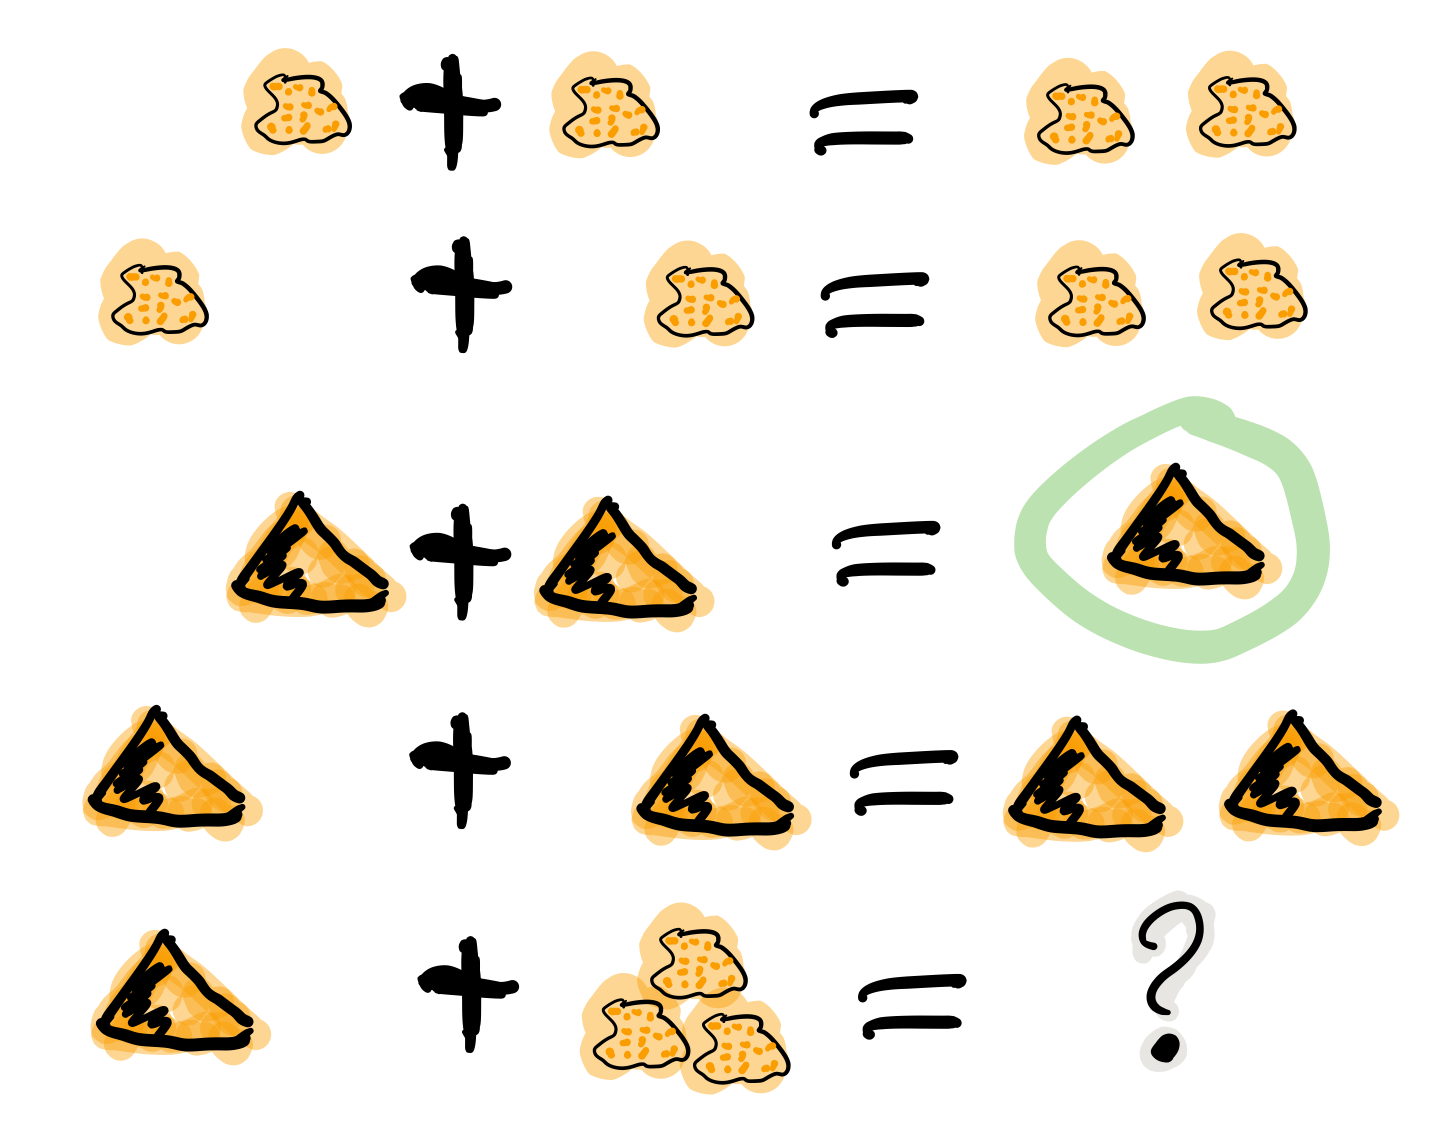
\includegraphics[width=4cm]{Sandpiles.png}}
  \caption{Sandpiles and sandgrains. The variety of equations depending on distance between addents.}
\end{figure}
When does a pile become a pile? The DRUHG answer it.

\section{Final remarks}
\epigraph{\raggedleft So many blissful revelations
\\Drawn by enlightenment's thought
\\And skill, the son of thoughest errors,
\\And genius, the paradoxes' pal,
\\And chance, the god-inventor.}{Alexander Pushkin, 1929}

A new clustering approach was introduced that provides: (i) a complete density-based clustering hierarchy; (ii) does not require parameters; (iii) a choice of metric defines near distances, that developes everything else. Philosophical investigation introduced a dialectical distance and birth of a true cluster. An experimental evaluation on a different datasets showed a state-of-the-art results. This work opens up a wide variety of future research: performance evaluations and improvements; discovery of attributes of dialectical distance and related MST-tree; and of course, philosophical battles over meaning of true cluster.

I could not finish it without a mentioning of the upcoming work. If we consider philosophical categories of Singular, Particular and Universal(S, P, U). Then we could derive the third phase of algorithm from the first two described in this work.  

\centerline{Phase I: $P of S = U$}
\centerline{Universal-Singular (connected tree)}
\vspace{\myvspace}
\centerline{Phase II: $S of U = P$}
\centerline{Particular-Universal (capacited cluster)}
\vspace{\myvspace}
\centerline{Phase III: $U of P = S$}
\centerline{Singular-Particular (shifted subject)}

In Phase III, all the interactions would inflict the shifting on a subject. Renewed subject would in turn relaunch the Phase I and so on. It would produce the Occam's automata. Hold tight for upcoming announcement and don't hesitate to contact(email is on the first page).

%%%%%%%%%%%%%%
% References %
%%%%%%%%%%%%%%

\printbibliography

\onecolumn

%%%%%%%%%%%%
% Appendix %
%%%%%%%%%%%%

\begin{appendices}
\section{On dialectics}\label{On dialectics}
The dialectics was first discovered by the Greeks. It was an art of dialog, it was a teaching of Becoming, it was a method. Every philosopher saw the surrounding duality and tried to describe it. My dialectics is a little bit different from others, and mainly based on the works of Hegel and Marx. I followed the first Marx's step and then kept the Hegelian system. To describe the resulted dialectics, I need to describe the works of these philosophers the way I see it. Then formalize my own vision of dialectical method. And the combination would be the DRUHG.

\subsection{Hegel's System of Logic}
This reading was painful, sometimes it took me a couple of hours to ger through one page. The book changes your thoughts, it is impossible to write afterwards, you will produce philosophical gibberish.
The System contains entities that are chained-nested into each other. 
It starts with a Being which is a Nothing. They are pulsing-changing each other. The Becoming taking them to the next level. Next level has it's own pulsing counter pair, and it's own bridge to the next level.
Like that Being turns to Essence, Essence turns to Concept, and so on until Absolute Idea comes along, and Absolute Idea give birth to Being.
Objective Idealism - the Idea rules them all.
Let's say I agree to all of that. But how do we get all of the world's diversity? We have the same Being which develops in the same manner and comes to the same begin.
What would happened if we had not one, but two, three, X Beings?
Hegel's driver is an internal contradictions of the entity.
What if the driver would be a relation between Beings?

\subsection{Marx's Capital}
Marx looks at the commodity and examines it as a relationship in society. Not as an entity! He noticed that Commodity has two pulsing sides exchange/use values. Those contradictory part do not cross. When you pay more you can get a worse quality.
Then instead of progressing to the next level he researches the ends of the relationship. The seller seeks exchange value and the buyer wants use value unless it's a pusher. And it happens to be that in a long chain from producer to a consumer most of the links don't care about the commodity and it's use value, all they want is to push it to the next in line. The people in links alienating the produce making it a commodity, alienating each other, and at the end alienating themselves.
Marx looked at the most common and most strangest of relationships between workers and employers. What is being sold there, what is the commodity of this relationship?
And he discovered that workers sell their work force and not the labor. The difference would be be a profit or surplus value.
Using this knowledge he built a two-circuit model which describes the Capitalism. Surplus value allows model to be a closed system. After several yearly cycle majority of the actors has to buy goods for the prices that includes surplus values but having wages without that value. This turns to Poverty, Wars and Crisises.
90\% of the work is the statistics and historical data, which was ok in 19th century, but is very boring in 21st.
Similarly to Hegel this book changes the way you think and write, you would be trying to subtly make fun of a rival just by citing him.
We could argue that surplus values turns to the Kapital hegelian style. Although, throughout his work Marx trolls people who thinks that the Kapital is real. Kapital is like a water funnel that grows and devours ships, no it is not. 

\subsection{Dialectics of negation}
The following is the formalization of negation used by Hegel and Marx.
\\ The meaning of something lies not only inside of that something but also outside in the surroundings.
\\ Differentiation from everything grants Beingness and uniqueness.
\\ The chair is a chair because it is \textit{not} a table, \textit{not} a wife, \textit{not} an universe, \textit{not} an all.
\\ The particle \textit{"not"} is negation, through it Being gets an outer side of it's meaning.

There are different types of negation.
\\ If you negate directly logically "not chair" turns to absolute infinity of everything and everyone minus that chair.
\\ Infinity without a one is still same infinity.
\\ "Not chair" equals to the World Infinity, "not wife" equals to the World Infinity, any not equates to it.
\\ Hegel called it the Absolute Spirit, by negating it you can get anything in the world.

Actually, by negating the Absolute Spirit Hegel would get Nothing, by negating Nothing he would get Being. 
\\ Didn't we agreed that we should be getting Absolute Spirit every time we negate something?
\\ In order to avoid that we should negate small. We need a negation that will keep us on the same level and allow us to return back.
\\ We need an inner negation that will reveal the other side of that thing.

Wife is someone who has a husband. The meaning of wife is outside of her it's in the husband.
\\ If you completely remove husband the wife won't be a wife.\footnote{Negating a chair is not breaking it. "Not" chair is a human's need in sitting. Aristotle.} Inner negation allows to get the other side of meaning. 
\\ Negating the wife we will get the husband. Negating the husband we'll get back the wife.
\\ "Not" wife is husband; "not" husband is wife; wife turns into husband and back; they are infinitely not-ing each other.
\\ This kind of infinite negation Hegel called Bad Infinity. This kind of "not" is fruitless.

Mutual negations are returning the contradiction and not giving any development.
\\ The next kind of negation will account that.
\\ The cycled contradictions are in unity and on a certain level of context.
\\ Negation can advance the unity to another entity if it will take into account that context.
\\ Bridge - a third member has to be added that unifies contradictions on their level and link to the next.
\\ Then it will be possible to negate the triad and reveal the next entity. This kind of negation will discard and keep the previous entities at the same time. It's called sublation.

Wife and husband are negated through the marriage and sublating to the family.
\\ Of course, these are not husband and wife but man and woman.
\\ Our language adapted to translate dialectics of intricacy of contradictions and context levels in single words.
\\ On one side it makes the life easier, on the other it interferes in our understanding of causes and effects.
\\ I'm forced to mention, that the contradictions are not being invented, they are there and we can reveal them if we try hard enough.

\subsection{Development}

Hegel looked at the Being and ignored the surroundings. His development came from within, from inner contradictions.
Such development is fruitless and creates the Bad Infinity which Hegel ironically disliked himself. Being turns to Essence then to Spirit and back to Being. It is instantaneous and lack the development.
\\ Marx took Hegel's method and used it to Commodity. Looked at it as a relationship not a thing in itself. 
Marx's first step was to find contradictions within the relationship. After that he researched the ends of the relationship and it's historical coming to be.
He didn't dialectically advanced further.

In my work I started like Marx, and continued like Hegel. Marxian research of created system is back-breaking labor for one person and up for a grab.
Unlike Hegel I looked at many Beings, their relationships are making them. Within them is nothing of matters.
The relationships are the key. Then like Marx I asked myself, what is the other side of relationship?
If you have feelings(or distance for metrics) what would be it complimentary part, it's inner negation?
And like that, I revealed the rankings. Continued in Marx steps I looked at the ends of the relationship, and revealed the Dialectical Distance.
\\ Unlike Marx I didn't have a historical evidences to back up my findings. Instead, I was following a goal - to not bring anything from the outside.
That forced me to use Hegelian method. Unlike Hegel's development of Being, Subjects formed real and not imaginary entities.

The formalization of negations allowed me to stay inside the theoretical boundaries. The hardest part was to understand the third member(Measure/Bridge). It is a secret sauce that brings qualitative jumps to the equation. Marx didn't need it for the historical research and ignored it overall. Hegel on the contrary had way too much to say. Measure takes a whole Section in a Science of Logic. 
\\ Compressed it reads: "In measure lies united abstractly expressed quality and quantity. Such quantity that it has certainty not in itself, but in other. Measure is self-correlated appearance. Some kind of reflection in self."
\\ Thus measure is almost a next entity. With measure, Subject count itself as a group. It act as it and for it, staying as subject.
\\ Product divided by sum gives such "outside" quantity. Same formula works in both phases and gives better results than the other expressions.

The final system does not hold any outer parameters and presents the clusters for what they really are - the interactions of submatter.
If you followed through this text you should be able to see that work is not over. And there are several directions to work with. Hegel's - to close the loop. Marx's - to research the system. Programmer's - to optimize the algorithm. Humankind's - to practice the truth.
\\ Good luck.

\newpage
\section{Pseudocode}\label{Pseudocode}
% мануал по псевдокоду http:\\mirror.ox.ac.uk/sites/ctan.org/macros/latex/contrib/algorithmicx/algorithmicx.pdf

DRUHG(\foreignlanguage{russian}{drug}): Dialectical Ranking Universal Hierarchical Grouper.
\\ The algorithm consists of two parts: Tree building and cluster detecting/labeling.
\\ The code part will be describing vanilla version and in between we will show tricks and speedups.  

To store the Tree we will be using union-find data structure aka merge-find set.\cite{ArticleReference10}
\\ To access neighbors we will be using KD-tree\cite{ArticleReference11} which allows to access k near neighbors. Small k would suffice - it is rarely needed to go through all pairs.

\begin{algorithm}
  \begin{algorithmic}[1]
    \Procedure {Pure reciprocity}{$Points$}: \Comment Adding pure reciprocal relation to the tree
      \ForAll {$p \in Points$}:
        \If {p's nearest neighbor has p as it's nearest}:
            \State Add the edge to the Tree 
            \State Weight = distance squared
        \EndIf
      \EndFor
    \EndProcedure
    \algstore{bkbreak}
  \end{algorithmic}
  \end{algorithm}

Those connections always precedes everything else. Even thou factual order would be broken. 
\\ In a sense algorithm is location-independent and separate Trees could be grown for a speed up. 

  \begin{algorithm}[h]
    \begin{algorithmic}[2]
      \algrestore{bkbreak}
      \Procedure {BuildMST}{$Points$}: \Comment Find minimal edge and connect to the Tree
        \Repeat
          
          \State Optimal = INF
          \State Edge = Null  
        
          \ForAll {$p \in Points$}:
            \ForAll {$nn \in p's neighbors$}:
              \If {p and nn are connected}:
                \State pass
              \EndIf
              \State R = rank of the nn in p's POV
              \State r = rank of the p in nn's POV
                
              \If {$R > r$}:
                \State pass
              \EndIf
              \State Equation = $r \cdot D^2 \cdot \sqrt{\frac{1+M}{M}}$:
                \State \indent D = distance from the point to the neighbor of rank r
                \State \indent M = how many neighbors the point has in the subtree limited by D
              \If {$Optimal < Equation$}:
                \State Optimal = Equation
                \State $Edge = (p, nn, D^2)$
              \EndIf
            \EndFor
          \EndFor
          \State Add Edge to the Tree
        \Until{all edges are connected in one tree}
        \State
        \Return {The Tree: ordered edges and weights}
      \EndProcedure
    \algstore{bkbreak}
\end{algorithmic}
\end{algorithm}

On the surface, we have bad vanilla's $O(n^2)$ time complexity. It can be easily improved - R($r\geq R$) and D are monotonically growing, meaning we don't have to go through all the neighbors.
Outside loop can be fixed with a heap\cite{ArticleReference12} structure.
\\ Those improvements decreases time complexity significantly.

\newpage
\begin{algorithm}[h]
  \begin{algorithmic}[3]
    \algrestore{bkbreak}
      
    \Procedure {LabelClusters}{$Tree$}: \Comment Labeling subtrees as clusters
      \State Limits(p) = 0
      \ForAll {edge(pair, weight) $/in$ Tree}:        
        \For {Left and Right subtrees}:
            \State $Border = K \cdot D^2 \cdot \sqrt{\frac{N \cdot N'}{N + N'}}$:
            \State \indent K = number of clusters in that subtree
            \State \indent $D^2$ = weight of the edge
            \State \indent N and N' = amount of points in subtrees
            \If {Border $\geq$ combined limit of subtree}:
              \State *That subtree is a cluster*
              \State It's $limit = N \cdot D^2$
            \EndIf
        \EndFor
        \State Merge subtrees: 
        \State \indent Add limits, number of clusters, number of points
      \EndFor
    \EndProcedure
  \end{algorithmic}
\end{algorithm}

Labeling is straight O(n) forward. It means that you could refeed the Tree if you want to get a different scopes.

\end{appendices}


\end{document}

% Create PDF on Linux:
% FILE=test; pkill -9 -f ${FILE} &>/dev/null; rm -f ${FILE}*aux ${FILE}*bbl ${FILE}*bib ${FILE}*blg ${FILE}*log ${FILE}*out ${FILE}*pdf &>/dev/null; pdflatex -halt-on-error ${FILE}; bibtex ${FILE} && pdflatex ${FILE} && pdflatex ${FILE} && (xdg-open ${FILE}.pdf &)